\documentclass[a4paper, 12pt, twoside]{report}
\usepackage[T1]{fontenc}
\usepackage[utf8]{inputenc}
\usepackage[italian]{babel}
\usepackage{geometry}
\usepackage{graphicx}
\usepackage{wrapfig2}
\usepackage{amsmath}
\usepackage{cancel} %semplificazione
\usepackage{amssymb}
\usepackage{amsthm} %teoremi e dimostrazioni e definizioni
\usepackage{gensymb} %simboli come ° = \degree  etc etc
\usepackage{cases}
\usepackage{subcaption}
\usepackage{hyperref}
\hypersetup{
	colorlinks=true,
	linkcolor=blue,    
	urlcolor=blue,
	%pdfpagemode=FullScreen,
}
\urlstyle{same}
\usepackage{color} % testo colorato
\raggedbottom
\setlength{\parindent}{0pt}
\usepackage{multirow}
\usepackage{booktabs} %tabelle scientifiche


%%%%%%%%%%%%%%%%%%%%%%%%%%%%%%%%%%%%%%%%%%%% AMBIENTE TIKZ 
\usepackage{tikz} %disegni e mappe
\usetikzlibrary{patterns}
\usepackage{pgfplots}
\pgfplotsset{compat=1.15}
\usepackage{mathrsfs}
\usetikzlibrary{arrows,decorations.markings,arrows.meta, decorations.text}
\usepackage{circuitikz}

\tikzset{immagine/.style={%
		above right, inner sep=0pt, outer sep=0pt},
	testo/.style={fill=white, align=center,
		fill opacity=0.6, text opacity=1, below,
		font=\sffamily\bfseries\footnotesize}}
	
%%%%%%%%%%%%%%%%%%%%%%%%%%%%%%%%%%%%%%%%%%%% SIUNITX 
\usepackage{siunitx}



%%%%%%%%%%%%%%%%%%%%%%%%%%%%%%%%%%%%%%%%%%%%%%%%%%%%%%%%% NUOVI COMANDI
\newcommand{\ra}[1]{\renewcommand{\arraystretch}{#1}} %stretcho le tabelle



\begin{document}
\begin{titlepage}
	\begin{center}
		
		
\includegraphics[width=0.8\textwidth]{figures/unitus_marchio_2020_DEIM}
		
		\vspace{0.5cm}
		
		{\Large Corso di Laurea in Ingegneria Industriale}
		
		\vspace{0.5cm}
		
		{\Large Laboratorio di Misure Meccaniche e Termiche}
		
		\vspace{0.5cm}
		
		{\Large A.A 2022-2023}
		
		\vspace{1.5cm}
		
		\textbf{{\Huge Relazione Esercitazione 2}}
		
		\vspace{0.5cm}
		{\LARGE Amplificatore operazionale}
		
		\vspace{1.5cm}
		
		\textbf{Andrea Marchegiani, Gruppo 3, mat. 810513}\\
		\href{mailto:andrea.marchegiani@studenti.unitus.it}{andrea.marchegiani@studenti.unitus.it} 
		
		
		\vfill
		
		
		
		28/11/2022
		
	\end{center}
\end{titlepage}
	
	
	\setcounterpageref{secnumdepth}{0}	
	\tableofcontents 
	\newpage
	
	
	\section{Amplificatore in configurazione invertente} 
	
	\begin{figure}[H]
		\centering
		\scalebox{1.2}{\begin{circuitikz}
				%\draw [help lines] (0,0) grid (10,10);			
				\draw (5,1) node[op amp, anchor=+] (OA1) {};    % Amplificatore
				\draw (OA1.+) -- (5,-0.5) node[ground]{};       % Ramo non invertente a terra
				\draw (OA1.-) to [R, l_=$R_i$] (3,2) to[european voltage source, l_=$V_i$] (3,0) -- (3,-0.5) node[ground]{}; % Ramo invertente col segnale
				\draw (OA1.-) -- (5,3) to [R, l^=$R_f$] (5,3 -| OA1.out) -- (OA1.out); % Ramo di feedback
				\draw (7.5,1) -- (7.5,-0.5) node[ground]{$V_{out}$};	% Uscita		
		\end{circuitikz}}
	\end{figure}
	
	Per il principio di massa virtuale 
	\[V_+ = V_-\]
	Ciò in prima approssimazione può considerarsi corretto perché:
	\begin{enumerate}
		\item Come la resistenza interna all'amplificatore aumenta, diminuirà la corrente che vi scorre attraverso e quindi la differenza di potenziale ai morsetti + e - si ridurrà fino a tendere a zero.
		\item Operativamente si osserva in uscita un segnale che non satura, allora nella relazione \[V_{out} = A(V_+-V_-)\] Si può porre \[A\rightarrow\infty \Rightarrow \Delta V\rightarrow0\] E quindi \[V_+\approx V_-\]
	\end{enumerate}
	
	Nel circuito chiuso invertente il morsetto + è posto a terra e quindi $V_+=0$, applicando il principio di massa virtuale si osserva così che:
	\[V_- = V_+ = 0\]
	La corrente che scorre su $R_i$ è
	\[I^* = {V_i-V_-\over R_i}\]
	Mentre quella che scorre su $R_f$ è 
	\[I^{**} = {V_--V_{out}\over R_f} \]
	Poiché la corrente sul circuito è la stessa, questi di contribuiti devono essere uguali, si ricava così
	\begin{equation}\label{eq:1}
		V_{out} = -{R_f\over R_i}V_i
	\end{equation}
	La quantità $\dfrac{R_f}{R_i}$ altro non è che il guadagno, l'entità con cui si amplifica o si deamplifica il segnale in ingresso, la pendenza della curva caratteristica ingresso - uscita. \newline 
	

	Similmente, per un circuito chiuso dove il segnale in ingresso è posto sul ramo non invertente (amplificatore non invertente), varrà 
	\[V_{out} = \left(1+\dfrac{R_f}{R_i}\right)V_i\]
	In questo caso il guadagno sarà sempre positivo e maggiore dell'unità per cui non sarà possibile deamplificare il segnale in ingresso.
			
	\begin{figure}[H]
		\centering
		\subfloat{\scalebox{0.6}{\begin{tikzpicture} 
					%\draw [help lines] (0,0) grid (10,10);
					\draw [->](5,0) -- (5,10) node [pos=1, left] {$V_{out}$};
					\draw [->](0,5) -- (10,5) node [pos=1, below] {$V_i$};
					\draw (5.5,9) -- (4.5,1) node[pos=0.75, left] {$1+\dfrac{R_f}{R_i}$};
					\draw (5.5,9) -- (10,9);
					\draw (4.5,1) -- (0,1);
					%Valori 
					\draw[dashed] (5,9) -- (8,9) node[pos=0, left] {$V_{Al}$};
					\draw[dashed] (5.5,5) -- (5.5,9) node[pos=0, below] {$V_{Lin}$};
					\node [draw] at (7.5,2.5) {{\footnotesize Amplificatore non invertente}};
		\end{tikzpicture}}} \quad \subfloat{\scalebox{0.6}{\begin{tikzpicture} 
					%\draw [help lines] (0,0) grid (10,10);
					\draw [->](5,0) -- (5,10) node [pos=1, left] {$V_{out}$};
					\draw [->](0,5) -- (10,5) node [pos=1, below] {$V_i$};
					\draw (6,1) -- (4,9) node[pos=0.75, left] {$-\dfrac{R_f}{R_i}$};
					\draw (4,9) -- (0,9);
					\draw (6,1) -- (10,1);
					%Valori 
					\draw[dashed] (5,9) -- (4,9) node[pos=0, right] {$V_{Al}$};
					\draw[dashed] (6,5) -- (6,1) node[pos=0, above] {$V_{Lin}$};
					\node [draw] at (2.5,2.5) {Amplificatore invertente};
		\end{tikzpicture}}}
	\end{figure}
	
	
\newpage

Ai fini dell'esperienza, per realizzare un amplificatore invertente dal guadano di $2.2$ si pone sul ramo di feedback una resistenza $R_f = \SI{2.2}{\kilo\ohm}$ mentre sul ramo invertente una resistenza di $R_i = \SI{1}{\kilo\ohm}$, in questo modo il guadagno teorico è pari a 
\[G^{th} = \dfrac{\SI{2.2}{\kilo\ohm}}{\SI{1}{\kilo\ohm}} = 2.2\]

\subsection{Quesito 1: determinare sperimentalmente il guadagno}
Se il segnale in \textcolor{cyan}{uscita} è \textcolor{cyan}{BLU} e quello in \textcolor{olive}{ingresso} è \textcolor{olive}{GIALLO} si può calcolare il guadagno sperimentale dalla (\ref{eq:1})
\[V_{out} = GV_i \Rightarrow G = \left|\dfrac{V_{out}}{V_i}\right|\]	
\begin{figure}[H]
	\centering
	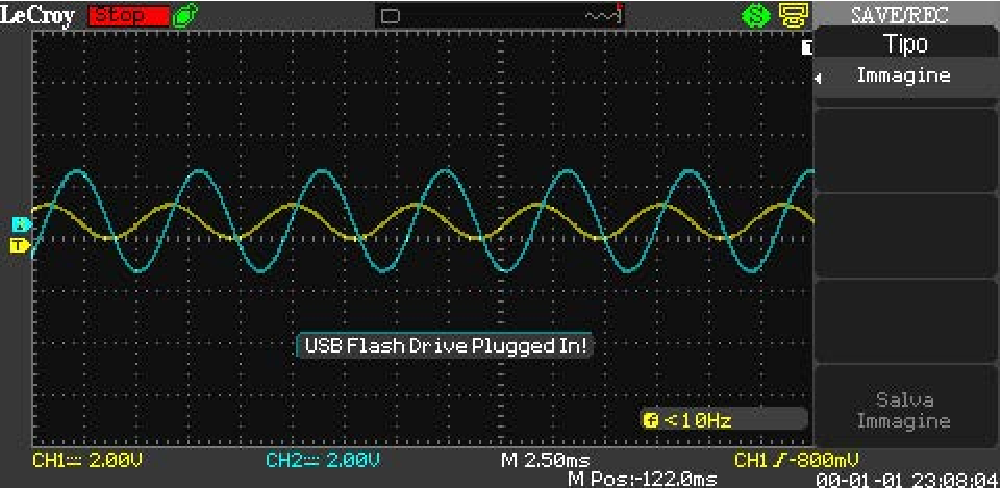
\includegraphics[width=0.7\linewidth]{imag/WA000017}
	\caption{Amplificatore invertente, valutazione sperimentale del guadagno}
	\label{fig:wa000017}
\end{figure}
Dall'oscilloscopio si legge che 
\[V_i = \SI{1.6}{\volt} \qquad V_{out} = \SI{3.9}{\volt}\]
Per cui 
\[G^{Re} = \dfrac{\SI{3.9}{\volt}}{\SI{1.6}{\volt}} = 2.4\]
Il segnale è deamplificato

\newpage

\subsection{Quesito 2: Per quale ampiezza teorica l'amplificatore va in saturazione?}

Per il teorema di non amplificazione, l'amplificatore va in saturazione quando in ingresso è applicato un segnale pari a quello di alimentazione dell'amplificatore stesso, che per l'amplificatore in esame ($\mu A741$) vale $V_{cc}=\SI{\pm15}{\volt}$. \newline

Per un amplificatore a circuito aperto si può scrivere
\[V_{out} = A(V_+-V_-)\]
In questo tipo di amplificatori il guadagno può raggiungere valori dell'ordine di $A = \num{e6}$, poiché il guadagno indica la pendenza della caratteristica ingresso - uscita, più il guadagno cresce più la retta diviene pendente, ciò significa avere una zona di linearità enormemente ridotta.
\begin{figure}[H]
	\centering
	\subfloat{\begin{circuitikz} \draw
		 (0,0) node[op amp] (opamp) {}
		 (opamp.+) node[left] {$V_+$}
		 (opamp.-) node[left] {$V_-$}
		 (opamp.out) node[right] {$V_{out}$}
		 (opamp.up) --++(0,0.5) node[vcc]{\textnormal{$V_{cc+}$}}
		 (opamp.down) --++(0,-0.5) node[vee]{\textnormal{$V_{cc-}$}}
		 ;
		\end{circuitikz}} \quad \subfloat{\scalebox{0.6}{\begin{tikzpicture} 
			%\draw [help lines] (0,0) grid (10,10);
			\draw [->](5,0) -- (5,10) node [pos=1, left] {$V_{out}$};
			\draw [->](0,5) -- (10,5) node [pos=1, below] {$V_+-V_-$};
			\draw (5.2,9) -- (4.8,1) node[pos=0.75, left] {$A$};
			\draw (5.2,9) -- (10,9);
			\draw (4.8,1) -- (0,1);
			%Valori 
			\draw[dashed] (5,9) -- (8,9) node[pos=0, left] {$V_{Al}$};
			\draw[dashed] (5.2,5) -- (5.2,9);
			\node at (5.5,4.6) {$V_{Lin}$};
			\node [draw] at (7.5,2.5) {{\footnotesize Circuito aperto}};
	\end{tikzpicture}}}
\end{figure}
Infatti per in circuito aperto varrebbe 
\[\Delta V_{Lin} = \dfrac{V_{cc}}{A} = \SI{15}{\micro\volt}\] 
Ciò significa che non appena la differenza di tensione in ingresso è di pochissimo superiore allo zero, il segnale satura alla tensione di alimentazione: è per questo che il circuito aperto non può essere usato come amplificatore (tuttalpiù come comparatore), proprio a causa del suo elevatissimo guadagno che limita fortemente la sua zona di linearità. 

\newpage

Al fine perciò di realizzare un amplificatore che permetta la corretta visualizzazione del segnale amplificato si decide di chiudere il circuito e applicare una retroazione: il segnale in uscita viene riportato all'ingresso mediante un ramo di feedback costituito da elementi passivi, che sebbene comporti un abbassamento del guadagno, permette di avere una zona di linearità maggiore, pur non eliminando del tutto il problema della saturazione.\newline 

Per rispondere al quesito:

L'ampiezza teorica di saturazione sarà
\[\Delta V^{th} = \dfrac{V_{cc}}{G^{th}} = \dfrac{\SI{15}{\volt}}{2.2} = \SI{6.81}{\volt}\]
Mentre quella sperimentale sarà
\[\Delta V^{Re} = \dfrac{V_{cc}}{G^{Re}} = \dfrac{\SI{15}{\volt}}{2.4} = \SI{6.25}{\volt}\]
Con un errore relativo pari a 
\[e \% = \dfrac{\Delta V^{Re}-\Delta V^{th}}{\Delta V^{Re}}\cdot100=8.2\%\]













\newpage
	\section{Filtro attivo passa alto non invertente}
	
	\begin{figure}[H]
		\centering
		\scalebox{1.2}{\begin{circuitikz}
				%\draw [help lines] (0,0) grid (10,10);			
				\draw (5,1) node[op amp, anchor=+] (OA1) {};    % Amplificatore
				\draw (OA1.+) to [R, l^=$R$] (5,-0.5) node[ground]{};       % Ramo non invertente 1 a terra
				\draw (OA1.+) to [C, l^=$C_i$] (3,1) to[european voltage source, l_=$V_i$] (3,-0.5) -- (3,-0.5) node[ground]{}; % Ramo non invertente 2 col segnale
				\draw (OA1.-) to [R, l_=$R_i$] (2,2) -- (2,-0.5) node[ground]{}; % Ramo invertente a terra
				\draw (OA1.-) -- (5,3) to [R, l^=$R_f$] (5,3 -| OA1.out) -- (OA1.out); % Ramo di feedback
				\draw (7.5,1) -- (7.5,-0.5) node[ground]{$V_{out}$};	% Uscita		
		\end{circuitikz}}
	\end{figure}
	Si nota immediatamente che $V_-=0$, per cui dall'uguaglianza della corrente che scorre sul ricruito si ricava
	\[-\dfrac{V_+}{R_i} = \dfrac{V_+-V_{out}}{R_f}\Rightarrow V_{out} = \left(1+\dfrac{R_f}{R_i}\right)V_+\]
	$V_+$ diviene calcolabile a partire dalla formula del partitore di corrente-
	\begin{figure}[H]
		\centering
		\scalebox{0.6}{\begin{circuitikz}
				%\draw [help lines] (0,0) grid (5,5);			
				\draw (0,0) to[european voltage source, l^=$V_i$] (0,5) -- (3,5) to [generic, l^=$Z_C$] (3,2.5) to [generic, l^=$Z_R$] (3,1) -- (3,0) -- (0,0); % Circuito 
				\draw (3,2.5) 	to [short, -*]	(5,2.5); 
				\draw (3,0.5) 	to [short, -*]	(5,0.5); 
				\draw (5,0.5)to[open,v_>=$V_+$,*-*](5,2.5);
		\end{circuitikz}}
	\end{figure}	
	\[V_+ = \dfrac{Z_R}{Z_R+Z_C}V_i= \dfrac{R}{R + \dfrac{1}{j\omega C}}V_i = \dfrac{j\omega RC}{1+j\omega RC}V_i\]
	Per cui
	\[V_{out} = \left(1+\dfrac{R_f}{R_i}\right)\dfrac{j\omega RC}{1+j\omega RC}V_i\]
	Il guadagno sarà sempre 
	\begin{equation}\label{eq:2}
		G = \left|\dfrac{V_{out}}{V_i}\right| = \left(1+\dfrac{R_f}{R_i}\right)\dfrac{\omega RC}{\sqrt{1+(\omega RC)^2}}
	\end{equation}
	Evidenziando un andamento del genere 
	\begin{figure}[H]
		\centering\definecolor{yqqqqq}{rgb}{0.5019607843137255,0.,0.}
		\begin{tikzpicture}[line cap=round,line join=round,>=triangle 45,x=1.0cm,y=1.0cm]
			\begin{axis}[
				x=3cm,y=3cm,
				axis lines=middle,
				ymajorgrids=true,
				xmajorgrids=true,
				xmin=0.0,
				xmax=4.0,
				ymin=0.0,
				ymax=1.5,
				ytick=\empty, xtick=\empty,
				xticklabels=\empty,yticklabels=\empty, extra y ticks={1}, extra y tick labels={$1+\dfrac{R_f}{R_i}$},
				xlabel=$\omega$, ylabel=$G$]
				\clip(0.,0.) rectangle (3.5,1.5);
				\draw[line width=2.pt,color=yqqqqq] (0.0,0.0) -- (0.0,0.0);
				\draw[line width=2.pt,color=yqqqqq] (0.0,0.0) -- (0.00875349125,0.008753155907225514);
				\draw[line width=2.pt,color=yqqqqq] (0.00875349125,0.008753155907225514) -- (0.0175034825,0.01750080182835431);
				\draw[line width=2.pt,color=yqqqqq] (0.0175034825,0.01750080182835431) -- (0.02625347375,0.0262444308880574);
				\draw[line width=2.pt,color=yqqqqq] (0.02625347375,0.0262444308880574) -- (0.035003465,0.034982040817788156);
				\draw[line width=2.pt,color=yqqqqq] (0.035003465,0.034982040817788156) -- (0.043753456249999996,0.04371163624330683);
				\draw[line width=2.pt,color=yqqqqq] (0.043753456249999996,0.04371163624330683) -- (0.052503447499999994,0.052431230953803795);
				\draw[line width=2.pt,color=yqqqqq] (0.052503447499999994,0.052431230953803795) -- (0.06125343874999999,0.061138850146626296);
				\draw[line width=2.pt,color=yqqqqq] (0.06125343874999999,0.061138850146626296) -- (0.07000342999999999,0.06983253264172995);
				\draw[line width=2.pt,color=yqqqqq] (0.07000342999999999,0.06983253264172995) -- (0.07875342125,0.07851033306012077);
				\draw[line width=2.pt,color=yqqqqq] (0.07875342125,0.07851033306012077) -- (0.0875034125,0.0871703239607237);
				\draw[line width=2.pt,color=yqqqqq] (0.0875034125,0.0871703239607237) -- (0.09625340375000001,0.09581059793030956);
				\draw[line width=2.pt,color=yqqqqq] (0.09625340375000001,0.09581059793030956) -- (0.10500339500000001,0.10442926962133213);
				\draw[line width=2.pt,color=yqqqqq] (0.10500339500000001,0.10442926962133213) -- (0.11375338625000002,0.1130244777327679);
				\draw[line width=2.pt,color=yqqqqq] (0.11375338625000002,0.1130244777327679) -- (0.12250337750000002,0.12159438692931425);
				\draw[line width=2.pt,color=yqqqqq] (0.12250337750000002,0.12159438692931425) -- (0.13125336875000002,0.13013718969458096);
				\draw[line width=2.pt,color=yqqqqq] (0.13125336875000002,0.13013718969458096) -- (0.14000336000000002,0.13865110811420817);
				\draw[line width=2.pt,color=yqqqqq] (0.14000336000000002,0.13865110811420817) -- (0.14875335125000003,0.14713439558515481);
				\draw[line width=2.pt,color=yqqqqq] (0.14875335125000003,0.14713439558515481) -- (0.15750334250000003,0.15558533844772568);
				\draw[line width=2.pt,color=yqqqqq] (0.15750334250000003,0.15558533844772568) -- (0.16625333375000004,0.16400225753723927);
				\draw[line width=2.pt,color=yqqqqq] (0.16625333375000004,0.16400225753723927) -- (0.17500332500000004,0.1723835096525802);
				\draw[line width=2.pt,color=yqqqqq] (0.17500332500000004,0.1723835096525802) -- (0.18375331625000005,0.18072748893922877);
				\draw[line width=2.pt,color=yqqqqq] (0.18375331625000005,0.18072748893922877) -- (0.19250330750000005,0.18903262818471048);
				\draw[line width=2.pt,color=yqqqqq] (0.19250330750000005,0.18903262818471048) -- (0.20125329875000006,0.1972974000247612);
				\draw[line width=2.pt,color=yqqqqq] (0.20125329875000006,0.1972974000247612) -- (0.21000329000000006,0.2055203180588571);
				\draw[line width=2.pt,color=yqqqqq] (0.21000329000000006,0.2055203180588571) -- (0.21875328125000007,0.21369993787410502);
				\draw[line width=2.pt,color=yqqqqq] (0.21875328125000007,0.21369993787410502) -- (0.22750327250000008,0.2218348579768372);
				\draw[line width=2.pt,color=yqqqqq] (0.22750327250000008,0.2218348579768372) -- (0.23625326375000008,0.22992372063158828);
				\draw[line width=2.pt,color=yqqqqq] (0.23625326375000008,0.22992372063158828) -- (0.2450032550000001,0.2379652126074661);
				\draw[line width=2.pt,color=yqqqqq] (0.2450032550000001,0.2379652126074661) -- (0.25375324625000006,0.2459580658322441);
				\draw[line width=2.pt,color=yqqqqq] (0.25375324625000006,0.2459580658322441) -- (0.26250323750000004,0.2539010579548148);
				\draw[line width=2.pt,color=yqqqqq] (0.26250323750000004,0.2539010579548148) -- (0.27125322875,0.26179301281693657);
				\draw[line width=2.pt,color=yqqqqq] (0.27125322875,0.26179301281693657) -- (0.28000322,0.26963280083548913);
				\draw[line width=2.pt,color=yqqqqq] (0.28000322,0.26963280083548913) -- (0.28875321125,0.27741933929671986);
				\draw[line width=2.pt,color=yqqqqq] (0.28875321125,0.27741933929671986) -- (0.29750320249999995,0.2851515925642119);
				\draw[line width=2.pt,color=yqqqqq] (0.29750320249999995,0.2851515925642119) -- (0.30625319374999993,0.2928285722025411);
				\draw[line width=2.pt,color=yqqqqq] (0.30625319374999993,0.2928285722025411) -- (0.3150031849999999,0.3004493370188031);
				\draw[line width=2.pt,color=yqqqqq] (0.3150031849999999,0.3004493370188031) -- (0.3237531762499999,0.30801299302439206);
				\draw[line width=2.pt,color=yqqqqq] (0.3237531762499999,0.30801299302439206) -- (0.33250316749999986,0.3155186933195919);
				\draw[line width=2.pt,color=yqqqqq] (0.33250316749999986,0.3155186933195919) -- (0.34125315874999984,0.32296563790370414);
				\draw[line width=2.pt,color=yqqqqq] (0.34125315874999984,0.32296563790370414) -- (0.3500031499999998,0.3303530734135779);
				\draw[line width=2.pt,color=yqqqqq] (0.3500031499999998,0.3303530734135779) -- (0.3587531412499998,0.3376802927935362);
				\draw[line width=2.pt,color=yqqqqq] (0.3587531412499998,0.3376802927935362) -- (0.3675031324999998,0.34494663489979654);
				\draw[line width=2.pt,color=yqqqqq] (0.3675031324999998,0.34494663489979654) -- (0.37625312374999975,0.35215148404257696);
				\draw[line width=2.pt,color=yqqqqq] (0.37625312374999975,0.35215148404257696) -- (0.38500311499999973,0.3592942694691451);
				\draw[line width=2.pt,color=yqqqqq] (0.38500311499999973,0.3592942694691451) -- (0.3937531062499997,0.36637446479112984);
				\draw[line width=2.pt,color=yqqqqq] (0.3937531062499997,0.36637446479112984) -- (0.4025030974999997,0.3733915873594482);
				\draw[line width=2.pt,color=yqqqqq] (0.4025030974999997,0.3733915873594482) -- (0.41125308874999966,0.38034519759022595);
				\draw[line width=2.pt,color=yqqqqq] (0.41125308874999966,0.38034519759022595) -- (0.42000307999999964,0.38723489824509605);
				\draw[line width=2.pt,color=yqqqqq] (0.42000307999999964,0.38723489824509605) -- (0.4287530712499996,0.3940603336692582);
				\draw[line width=2.pt,color=yqqqqq] (0.4287530712499996,0.3940603336692582) -- (0.4375030624999996,0.4008211889906547);
				\draw[line width=2.pt,color=yqqqqq] (0.4375030624999996,0.4008211889906547) -- (0.4462530537499996,0.4075171892835943);
				\draw[line width=2.pt,color=yqqqqq] (0.4462530537499996,0.4075171892835943) -- (0.45500304499999955,0.4141480987001056);
				\draw[line width=2.pt,color=yqqqqq] (0.45500304499999955,0.4141480987001056) -- (0.46375303624999953,0.4207137195722508);
				\draw[line width=2.pt,color=yqqqqq] (0.46375303624999953,0.4207137195722508) -- (0.4725030274999995,0.4272138914885647);
				\draw[line width=2.pt,color=yqqqqq] (0.4725030274999995,0.4272138914885647) -- (0.4812530187499995,0.4336484903477097);
				\draw[line width=2.pt,color=yqqqqq] (0.4812530187499995,0.4336484903477097) -- (0.49000300999999946,0.44001742739235694);
				\draw[line width=2.pt,color=yqqqqq] (0.49000300999999946,0.44001742739235694) -- (0.49875300124999944,0.44632064822621653);
				\draw[line width=2.pt,color=yqqqqq] (0.49875300124999944,0.44632064822621653) -- (0.5075029924999994,0.4525581318170409);
				\draw[line width=2.pt,color=yqqqqq] (0.5075029924999994,0.4525581318170409) -- (0.5162529837499994,0.45872988948832955);
				\draw[line width=2.pt,color=yqqqqq] (0.5162529837499994,0.45872988948832955) -- (0.5250029749999994,0.4648359639023536);
				\draw[line width=2.pt,color=yqqqqq] (0.5250029749999994,0.4648359639023536) -- (0.5337529662499993,0.4708764280370152);
				\draw[line width=2.pt,color=yqqqqq] (0.5337529662499993,0.4708764280370152) -- (0.5425029574999993,0.47685138415893863);
				\draw[line width=2.pt,color=yqqqqq] (0.5425029574999993,0.47685138415893863) -- (0.5512529487499993,0.48276096279508157);
				\draw[line width=2.pt,color=yqqqqq] (0.5512529487499993,0.48276096279508157) -- (0.5600029399999993,0.48860532170503423);
				\draw[line width=2.pt,color=yqqqqq] (0.5600029399999993,0.48860532170503423) -- (0.5687529312499993,0.49438464485606054);
				\draw[line width=2.pt,color=yqqqqq] (0.5687529312499993,0.49438464485606054) -- (0.5775029224999992,0.500099141402816);
				\draw[line width=2.pt,color=yqqqqq] (0.5775029224999992,0.500099141402816) -- (0.5862529137499992,0.5057490446735606);
				\draw[line width=2.pt,color=yqqqqq] (0.5862529137499992,0.5057490446735606) -- (0.5950029049999992,0.5113346111645688);
				\draw[line width=2.pt,color=yqqqqq] (0.5950029049999992,0.5113346111645688) -- (0.6037528962499992,0.5168561195443214);
				\draw[line width=2.pt,color=yqqqqq] (0.6037528962499992,0.5168561195443214) -- (0.6125028874999991,0.5223138696689549);
				\draw[line width=2.pt,color=yqqqqq] (0.6125028874999991,0.5223138696689549) -- (0.6212528787499991,0.5277081816103241);
				\draw[line width=2.pt,color=yqqqqq] (0.6212528787499991,0.5277081816103241) -- (0.6300028699999991,0.5330393946979346);
				\draw[line width=2.pt,color=yqqqqq] (0.6300028699999991,0.5330393946979346) -- (0.6387528612499991,0.5383078665758854);
				\draw[line width=2.pt,color=yqqqqq] (0.6387528612499991,0.5383078665758854) -- (0.6475028524999991,0.5435139722758635);
				\draw[line width=2.pt,color=yqqqqq] (0.6475028524999991,0.5435139722758635) -- (0.656252843749999,0.5486581033071308);
				\draw[line width=2.pt,color=yqqqqq] (0.656252843749999,0.5486581033071308) -- (0.665002834999999,0.5537406667643453);
				\draw[line width=2.pt,color=yqqqqq] (0.665002834999999,0.5537406667643453) -- (0.673752826249999,0.5587620844539639);
				\draw[line width=2.pt,color=yqqqqq] (0.673752826249999,0.5587620844539639) -- (0.682502817499999,0.5637227920398873);
				\draw[line width=2.pt,color=yqqqqq] (0.682502817499999,0.5637227920398873) -- (0.691252808749999,0.5686232382089174);
				\draw[line width=2.pt,color=yqqqqq] (0.691252808749999,0.5686232382089174) -- (0.7000027999999989,0.5734638838565166);
				\draw[line width=2.pt,color=yqqqqq] (0.7000027999999989,0.5734638838565166) -- (0.7087527912499989,0.5782452012932814);
				\draw[line width=2.pt,color=yqqqqq] (0.7087527912499989,0.5782452012932814) -- (0.7175027824999989,0.5829676734724643);
				\draw[line width=2.pt,color=yqqqqq] (0.7175027824999989,0.5829676734724643) -- (0.7262527737499989,0.5876317932388099);
				\draw[line width=2.pt,color=yqqqqq] (0.7262527737499989,0.5876317932388099) -- (0.7350027649999988,0.5922380625989057);
				\draw[line width=2.pt,color=yqqqqq] (0.7350027649999988,0.5922380625989057) -- (0.7437527562499988,0.5967869920131799);
				\draw[line width=2.pt,color=yqqqqq] (0.7437527562499988,0.5967869920131799) -- (0.7525027474999988,0.6012790997096255);
				\draw[line width=2.pt,color=yqqqqq] (0.7525027474999988,0.6012790997096255) -- (0.7612527387499988,0.60571491101927);
				\draw[line width=2.pt,color=yqqqqq] (0.7612527387499988,0.60571491101927) -- (0.7700027299999987,0.6100949577333621);
				\draw[line width=2.pt,color=yqqqqq] (0.7700027299999987,0.6100949577333621) -- (0.7787527212499987,0.6144197774821955);
				\draw[line width=2.pt,color=yqqqqq] (0.7787527212499987,0.6144197774821955) -- (0.7875027124999987,0.618689913135448);
				\draw[line width=2.pt,color=yqqqqq] (0.7875027124999987,0.618689913135448) -- (0.7962527037499987,0.6229059122238726);
				\draw[line width=2.pt,color=yqqqqq] (0.7962527037499987,0.6229059122238726) -- (0.8050026949999987,0.6270683263821386);
				\draw[line width=2.pt,color=yqqqqq] (0.8050026949999987,0.6270683263821386) -- (0.8137526862499986,0.6311777108125862);
				\draw[line width=2.pt,color=yqqqqq] (0.8137526862499986,0.6311777108125862) -- (0.8225026774999986,0.6352346237696306);
				\draw[line width=2.pt,color=yqqqqq] (0.8225026774999986,0.6352346237696306) -- (0.8312526687499986,0.6392396260645155);
				\draw[line width=2.pt,color=yqqqqq] (0.8312526687499986,0.6392396260645155) -- (0.8400026599999986,0.6431932805900984);
				\draw[line width=2.pt,color=yqqqqq] (0.8400026599999986,0.6431932805900984) -- (0.8487526512499985,0.647096151865323);
				\draw[line width=2.pt,color=yqqqqq] (0.8487526512499985,0.647096151865323) -- (0.8575026424999985,0.6509488055990124);
				\draw[line width=2.pt,color=yqqqqq] (0.8575026424999985,0.6509488055990124) -- (0.8662526337499985,0.6547518082726028);
				\draw[line width=2.pt,color=yqqqqq] (0.8662526337499985,0.6547518082726028) -- (0.8750026249999985,0.65850572674142);
				\draw[line width=2.pt,color=yqqqqq] (0.8750026249999985,0.65850572674142) -- (0.8837526162499985,0.6622111278540853);
				\draw[line width=2.pt,color=yqqqqq] (0.8837526162499985,0.6622111278540853) -- (0.8925026074999984,0.6658685780896297);
				\draw[line width=2.pt,color=yqqqqq] (0.8925026074999984,0.6658685780896297) -- (0.9012525987499984,0.6694786432118857);
				\draw[line width=2.pt,color=yqqqqq] (0.9012525987499984,0.6694786432118857) -- (0.9100025899999984,0.6730418879407132);
				\draw[line width=2.pt,color=yqqqqq] (0.9100025899999984,0.6730418879407132) -- (0.9187525812499984,0.6765588756396185);
				\draw[line width=2.pt,color=yqqqqq] (0.9187525812499984,0.6765588756396185) -- (0.9275025724999983,0.6800301680193124);
				\draw[line width=2.pt,color=yqqqqq] (0.9275025724999983,0.6800301680193124) -- (0.9362525637499983,0.683456324856758);
				\draw[line width=2.pt,color=yqqqqq] (0.9362525637499983,0.683456324856758) -- (0.9450025549999983,0.6868379037292519);
				\draw[line width=2.pt,color=yqqqqq] (0.9450025549999983,0.6868379037292519) -- (0.9537525462499983,0.6901754597630839);
				\draw[line width=2.pt,color=yqqqqq] (0.9537525462499983,0.6901754597630839) -- (0.9625025374999983,0.6934695453963249);
				\draw[line width=2.pt,color=yqqqqq] (0.9625025374999983,0.6934695453963249) -- (0.9712525287499982,0.6967207101552864);
				\draw[line width=2.pt,color=yqqqqq] (0.9712525287499982,0.6967207101552864) -- (0.9800025199999982,0.6999295004442073);
				\draw[line width=2.pt,color=yqqqqq] (0.9800025199999982,0.6999295004442073) -- (0.9887525112499982,0.7030964593477211);
				\draw[line width=2.pt,color=yqqqqq] (0.9887525112499982,0.7030964593477211) -- (0.9975025024999982,0.706222126445663);
				\draw[line width=2.pt,color=yqqqqq] (0.9975025024999982,0.706222126445663) -- (1.0062524937499981,0.7093070376397829);
				\draw[line width=2.pt,color=yqqqqq] (1.0062524937499981,0.7093070376397829) -- (1.0150024849999981,0.712351724991936);
				\draw[line width=2.pt,color=yqqqqq] (1.0150024849999981,0.712351724991936) -- (1.023752476249998,0.7153567165733266);
				\draw[line width=2.pt,color=yqqqqq] (1.023752476249998,0.7153567165733266) -- (1.032502467499998,0.7183225363243924);
				\draw[line width=2.pt,color=yqqqqq] (1.032502467499998,0.7183225363243924) -- (1.041252458749998,0.7212497039249199);
				\draw[line width=2.pt,color=yqqqqq] (1.041252458749998,0.7212497039249199) -- (1.050002449999998,0.7241387346739929);
				\draw[line width=2.pt,color=yqqqqq] (1.050002449999998,0.7241387346739929) -- (1.058752441249998,0.7269901393793807);
				\draw[line width=2.pt,color=yqqqqq] (1.058752441249998,0.7269901393793807) -- (1.067502432499998,0.7298044242559858);
				\draw[line width=2.pt,color=yqqqqq] (1.067502432499998,0.7298044242559858) -- (1.076252423749998,0.7325820908329745);
				\draw[line width=2.pt,color=yqqqqq] (1.076252423749998,0.7325820908329745) -- (1.085002414999998,0.7353236358692288);
				\draw[line width=2.pt,color=yqqqqq] (1.085002414999998,0.7353236358692288) -- (1.093752406249998,0.7380295512767587);
				\draw[line width=2.pt,color=yqqqqq] (1.093752406249998,0.7380295512767587) -- (1.102502397499998,0.7407003240517367);
				\draw[line width=2.pt,color=yqqqqq] (1.102502397499998,0.7407003240517367) -- (1.1112523887499979,0.7433364362128074);
				\draw[line width=2.pt,color=yqqqqq] (1.1112523887499979,0.7433364362128074) -- (1.1200023799999979,0.7459383647463539);
				\draw[line width=2.pt,color=yqqqqq] (1.1200023799999979,0.7459383647463539) -- (1.1287523712499978,0.7485065815583963);
				\draw[line width=2.pt,color=yqqqqq] (1.1287523712499978,0.7485065815583963) -- (1.1375023624999978,0.7510415534328185);
				\draw[line width=2.pt,color=yqqqqq] (1.1375023624999978,0.7510415534328185) -- (1.1462523537499978,0.7535437419956187);
				\draw[line width=2.pt,color=yqqqqq] (1.1462523537499978,0.7535437419956187) -- (1.1550023449999978,0.7560136036849004);
				\draw[line width=2.pt,color=yqqqqq] (1.1550023449999978,0.7560136036849004) -- (1.1637523362499977,0.7584515897263177);
				\draw[line width=2.pt,color=yqqqqq] (1.1637523362499977,0.7584515897263177) -- (1.1725023274999977,0.7608581461137057);
				\draw[line width=2.pt,color=yqqqqq] (1.1725023274999977,0.7608581461137057) -- (1.1812523187499977,0.7632337135946351);
				\draw[line width=2.pt,color=yqqqqq] (1.1812523187499977,0.7632337135946351) -- (1.1900023099999977,0.7655787276606357);
				\draw[line width=2.pt,color=yqqqqq] (1.1900023099999977,0.7655787276606357) -- (1.1987523012499977,0.7678936185418441);
				\draw[line width=2.pt,color=yqqqqq] (1.1987523012499977,0.7678936185418441) -- (1.2075022924999976,0.7701788112058442);
				\draw[line width=2.pt,color=yqqqqq] (1.2075022924999976,0.7701788112058442) -- (1.2162522837499976,0.7724347253604663);
				\draw[line width=2.pt,color=yqqqqq] (1.2162522837499976,0.7724347253604663) -- (1.2250022749999976,0.7746617754603331);
				\draw[line width=2.pt,color=yqqqqq] (1.2250022749999976,0.7746617754603331) -- (1.2337522662499976,0.7768603707169366);
				\draw[line width=2.pt,color=yqqqqq] (1.2337522662499976,0.7768603707169366) -- (1.2425022574999975,0.7790309151120475);
				\draw[line width=2.pt,color=yqqqqq] (1.2425022574999975,0.7790309151120475) -- (1.2512522487499975,0.7811738074142593);
				\draw[line width=2.pt,color=yqqqqq] (1.2512522487499975,0.7811738074142593) -- (1.2600022399999975,0.7832894411984824);
				\draw[line width=2.pt,color=yqqqqq] (1.2600022399999975,0.7832894411984824) -- (1.2687522312499975,0.7853782048682066);
				\draw[line width=2.pt,color=yqqqqq] (1.2687522312499975,0.7853782048682066) -- (1.2775022224999975,0.7874404816803618);
				\draw[line width=2.pt,color=yqqqqq] (1.2775022224999975,0.7874404816803618) -- (1.2862522137499974,0.7894766497726097);
				\draw[line width=2.pt,color=yqqqqq] (1.2862522137499974,0.7894766497726097) -- (1.2950022049999974,0.7914870821929104);
				\draw[line width=2.pt,color=yqqqqq] (1.2950022049999974,0.7914870821929104) -- (1.3037521962499974,0.7934721469312102);
				\draw[line width=2.pt,color=yqqqqq] (1.3037521962499974,0.7934721469312102) -- (1.3125021874999974,0.795432206953106);
				\draw[line width=2.pt,color=yqqqqq] (1.3125021874999974,0.795432206953106) -- (1.3212521787499973,0.7973676202353489);
				\draw[line width=2.pt,color=yqqqqq] (1.3212521787499973,0.7973676202353489) -- (1.3300021699999973,0.7992787398030521);
				\draw[line width=2.pt,color=yqqqqq] (1.3300021699999973,0.7992787398030521) -- (1.3387521612499973,0.8011659137684777);
				\draw[line width=2.pt,color=yqqqqq] (1.3387521612499973,0.8011659137684777) -- (1.3475021524999973,0.8030294853712809);
				\draw[line width=2.pt,color=yqqqqq] (1.3475021524999973,0.8030294853712809) -- (1.3562521437499973,0.8048697930200958);
				\draw[line width=2.pt,color=yqqqqq] (1.3562521437499973,0.8048697930200958) -- (1.3650021349999972,0.8066871703353518);
				\draw[line width=2.pt,color=yqqqqq] (1.3650021349999972,0.8066871703353518) -- (1.3737521262499972,0.8084819461932186);
				\draw[line width=2.pt,color=yqqqqq] (1.3737521262499972,0.8084819461932186) -- (1.3825021174999972,0.8102544447705742);
				\draw[line width=2.pt,color=yqqqqq] (1.3825021174999972,0.8102544447705742) -- (1.3912521087499972,0.812004985590907);
				\draw[line width=2.pt,color=yqqqqq] (1.3912521087499972,0.812004985590907) -- (1.4000020999999971,0.8137338835710548);
				\draw[line width=2.pt,color=yqqqqq] (1.4000020999999971,0.8137338835710548) -- (1.4087520912499971,0.8154414490687002);
				\draw[line width=2.pt,color=yqqqqq] (1.4087520912499971,0.8154414490687002) -- (1.417502082499997,0.8171279879305369);
				\draw[line width=2.pt,color=yqqqqq] (1.417502082499997,0.8171279879305369) -- (1.426252073749997,0.8187938015410291);
				\draw[line width=2.pt,color=yqqqqq] (1.426252073749997,0.8187938015410291) -- (1.435002064999997,0.8204391868716924);
				\draw[line width=2.pt,color=yqqqqq] (1.435002064999997,0.8204391868716924) -- (1.443752056249997,0.8220644365308244);
				\draw[line width=2.pt,color=yqqqqq] (1.443752056249997,0.8220644365308244) -- (1.452502047499997,0.823669838813618);
				\draw[line width=2.pt,color=yqqqqq] (1.452502047499997,0.823669838813618) -- (1.461252038749997,0.8252556777525967);
				\draw[line width=2.pt,color=yqqqqq] (1.461252038749997,0.8252556777525967) -- (1.470002029999997,0.8268222331683109);
				\draw[line width=2.pt,color=yqqqqq] (1.470002029999997,0.8268222331683109) -- (1.478752021249997,0.8283697807202386);
				\draw[line width=2.pt,color=yqqqqq] (1.478752021249997,0.8283697807202386) -- (1.487502012499997,0.8298985919578384);
				\draw[line width=2.pt,color=yqqqqq] (1.487502012499997,0.8298985919578384) -- (1.496252003749997,0.8314089343717047);
				\draw[line width=2.pt,color=yqqqqq] (1.496252003749997,0.8314089343717047) -- (1.5050019949999969,0.8329010714447765);
				\draw[line width=2.pt,color=yqqqqq] (1.5050019949999969,0.8329010714447765) -- (1.5137519862499969,0.8343752627035566);
				\draw[line width=2.pt,color=yqqqqq] (1.5137519862499969,0.8343752627035566) -- (1.5225019774999968,0.8358317637692982);
				\draw[line width=2.pt,color=yqqqqq] (1.5225019774999968,0.8358317637692982) -- (1.5312519687499968,0.8372708264091213);
				\draw[line width=2.pt,color=yqqqqq] (1.5312519687499968,0.8372708264091213) -- (1.5400019599999968,0.8386926985870181);
				\draw[line width=2.pt,color=yqqqqq] (1.5400019599999968,0.8386926985870181) -- (1.5487519512499968,0.8400976245147176);
				\draw[line width=2.pt,color=yqqqqq] (1.5487519512499968,0.8400976245147176) -- (1.5575019424999967,0.8414858447023724);
				\draw[line width=2.pt,color=yqqqqq] (1.5575019424999967,0.8414858447023724) -- (1.5662519337499967,0.8428575960090401);
				\draw[line width=2.pt,color=yqqqqq] (1.5662519337499967,0.8428575960090401) -- (1.5750019249999967,0.844213111692929);
				\draw[line width=2.pt,color=yqqqqq] (1.5750019249999967,0.844213111692929) -- (1.5837519162499967,0.8455526214613829);
				\draw[line width=2.pt,color=yqqqqq] (1.5837519162499967,0.8455526214613829) -- (1.5925019074999966,0.8468763515205793);
				\draw[line width=2.pt,color=yqqqqq] (1.5925019074999966,0.8468763515205793) -- (1.6012518987499966,0.8481845246249182);
				\draw[line width=2.pt,color=yqqqqq] (1.6012518987499966,0.8481845246249182) -- (1.6100018899999966,0.8494773601260799);
				\draw[line width=2.pt,color=yqqqqq] (1.6100018899999966,0.8494773601260799) -- (1.6187518812499966,0.8507550740217326);
				\draw[line width=2.pt,color=yqqqqq] (1.6187518812499966,0.8507550740217326) -- (1.6275018724999966,0.8520178790038702);
				\draw[line width=2.pt,color=yqqqqq] (1.6275018724999966,0.8520178790038702) -- (1.6362518637499965,0.8532659845067655);
				\draw[line width=2.pt,color=yqqqqq] (1.6362518637499965,0.8532659845067655) -- (1.6450018549999965,0.8544995967545205);
				\draw[line width=2.pt,color=yqqqqq] (1.6450018549999965,0.8544995967545205) -- (1.6537518462499965,0.8557189188082017);
				\draw[line width=2.pt,color=yqqqqq] (1.6537518462499965,0.8557189188082017) -- (1.6625018374999965,0.8569241506125465);
				\draw[line width=2.pt,color=yqqqqq] (1.6625018374999965,0.8569241506125465) -- (1.6712518287499964,0.8581154890422277);
				\draw[line width=2.pt,color=yqqqqq] (1.6712518287499964,0.8581154890422277) -- (1.6800018199999964,0.8592931279476688);
				\draw[line width=2.pt,color=yqqqqq] (1.6800018199999964,0.8592931279476688) -- (1.6887518112499964,0.8604572582003949);
				\draw[line width=2.pt,color=yqqqqq] (1.6887518112499964,0.8604572582003949) -- (1.6975018024999964,0.8616080677379158);
				\draw[line width=2.pt,color=yqqqqq] (1.6975018024999964,0.8616080677379158) -- (1.7062517937499964,0.8627457416081297);
				\draw[line width=2.pt,color=yqqqqq] (1.7062517937499964,0.8627457416081297) -- (1.7150017849999963,0.8638704620132426);
				\draw[line width=2.pt,color=yqqqqq] (1.7150017849999963,0.8638704620132426) -- (1.7237517762499963,0.8649824083531962);
				\draw[line width=2.pt,color=yqqqqq] (1.7237517762499963,0.8649824083531962) -- (1.7325017674999963,0.8660817572685997);
				\draw[line width=2.pt,color=yqqqqq] (1.7325017674999963,0.8660817572685997) -- (1.7412517587499963,0.8671686826831594);
				\draw[line width=2.pt,color=yqqqqq] (1.7412517587499963,0.8671686826831594) -- (1.7500017499999962,0.8682433558456059);
				\draw[line width=2.pt,color=yqqqqq] (1.7500017499999962,0.8682433558456059) -- (1.7587517412499962,0.8693059453711102);
				\draw[line width=2.pt,color=yqqqqq] (1.7587517412499962,0.8693059453711102) -- (1.7675017324999962,0.8703566172821909);
				\draw[line width=2.pt,color=yqqqqq] (1.7675017324999962,0.8703566172821909) -- (1.7762517237499962,0.8713955350491085);
				\draw[line width=2.pt,color=yqqqqq] (1.7762517237499962,0.8713955350491085) -- (1.7850017149999962,0.8724228596297455);
				\draw[line width=2.pt,color=yqqqqq] (1.7850017149999962,0.8724228596297455) -- (1.7937517062499961,0.8734387495089702);
				\draw[line width=2.pt,color=yqqqqq] (1.7937517062499961,0.8734387495089702) -- (1.8025016974999961,0.8744433607374884);
				\draw[line width=2.pt,color=yqqqqq] (1.8025016974999961,0.8744433607374884) -- (1.811251688749996,0.8754368469701762);
				\draw[line width=2.pt,color=yqqqqq] (1.811251688749996,0.8754368469701762) -- (1.820001679999996,0.8764193595038995);
				\draw[line width=2.pt,color=yqqqqq] (1.820001679999996,0.8764193595038995) -- (1.828751671249996,0.8773910473148205);
				\draw[line width=2.pt,color=yqqqqq] (1.828751671249996,0.8773910473148205) -- (1.837501662499996,0.8783520570951896);
				\draw[line width=2.pt,color=yqqqqq] (1.837501662499996,0.8783520570951896) -- (1.846251653749996,0.8793025332896285);
				\draw[line width=2.pt,color=yqqqqq] (1.846251653749996,0.8793025332896285) -- (1.855001644999996,0.8802426181309021);
				\draw[line width=2.pt,color=yqqqqq] (1.855001644999996,0.8802426181309021) -- (1.863751636249996,0.8811724516751854);
				\draw[line width=2.pt,color=yqqqqq] (1.863751636249996,0.8811724516751854) -- (1.872501627499996,0.8820921718368261);
				\draw[line width=2.pt,color=yqqqqq] (1.872501627499996,0.8820921718368261) -- (1.881251618749996,0.8830019144226053);
				\draw[line width=2.pt,color=yqqqqq] (1.881251618749996,0.8830019144226053) -- (1.890001609999996,0.8839018131655004);
				\draw[line width=2.pt,color=yqqqqq] (1.890001609999996,0.8839018131655004) -- (1.8987516012499959,0.8847919997579531);
				\draw[line width=2.pt,color=yqqqqq] (1.8987516012499959,0.8847919997579531) -- (1.9075015924999958,0.8856726038846471);
				\draw[line width=2.pt,color=yqqqqq] (1.9075015924999958,0.8856726038846471) -- (1.9162515837499958,0.886543753254797);
				\draw[line width=2.pt,color=yqqqqq] (1.9162515837499958,0.886543753254797) -- (1.9250015749999958,0.887405573633954);
				\draw[line width=2.pt,color=yqqqqq] (1.9250015749999958,0.887405573633954) -- (1.9337515662499958,0.888258188875334);
				\draw[line width=2.pt,color=yqqqqq] (1.9337515662499958,0.888258188875334) -- (1.9425015574999958,0.8891017209506671);
				\draw[line width=2.pt,color=yqqqqq] (1.9425015574999958,0.8891017209506671) -- (1.9512515487499957,0.8899362899805802);
				\draw[line width=2.pt,color=yqqqqq] (1.9512515487499957,0.8899362899805802) -- (1.9600015399999957,0.8907620142645098);
				\draw[line width=2.pt,color=yqqqqq] (1.9600015399999957,0.8907620142645098) -- (1.9687515312499957,0.8915790103101568);
				\draw[line width=2.pt,color=yqqqqq] (1.9687515312499957,0.8915790103101568) -- (1.9775015224999957,0.8923873928624815);
				\draw[line width=2.pt,color=yqqqqq] (1.9775015224999957,0.8923873928624815) -- (1.9862515137499956,0.8931872749322477);
				\draw[line width=2.pt,color=yqqqqq] (1.9862515137499956,0.8931872749322477) -- (1.9950015049999956,0.8939787678241213);
				\draw[line width=2.pt,color=yqqqqq] (1.9950015049999956,0.8939787678241213) -- (2.0037514962499956,0.8947619811643236);
				\draw[line width=2.pt,color=yqqqqq] (2.0037514962499956,0.8947619811643236) -- (2.012501487499996,0.8955370229278515);
				\draw[line width=2.pt,color=yqqqqq] (2.012501487499996,0.8955370229278515) -- (2.021251478749996,0.8963039994652617);
				\draw[line width=2.pt,color=yqqqqq] (2.021251478749996,0.8963039994652617) -- (2.030001469999996,0.8970630155290324);
				\draw[line width=2.pt,color=yqqqqq] (2.030001469999996,0.8970630155290324) -- (2.0387514612499964,0.8978141742995007);
				\draw[line width=2.pt,color=yqqqqq] (2.0387514612499964,0.8978141742995007) -- (2.0475014524999966,0.8985575774103843);
				\draw[line width=2.pt,color=yqqqqq] (2.0475014524999966,0.8985575774103843) -- (2.056251443749997,0.8992933249738932);
				\draw[line width=2.pt,color=yqqqqq] (2.056251443749997,0.8992933249738932) -- (2.065001434999997,0.9000215156054353);
				\draw[line width=2.pt,color=yqqqqq] (2.065001434999997,0.9000215156054353) -- (2.073751426249997,0.9007422464479206);
				\draw[line width=2.pt,color=yqqqqq] (2.073751426249997,0.9007422464479206) -- (2.0825014174999974,0.9014556131956719);
				\draw[line width=2.pt,color=yqqqqq] (2.0825014174999974,0.9014556131956719) -- (2.0912514087499976,0.9021617101179458);
				\draw[line width=2.pt,color=yqqqqq] (2.0912514087499976,0.9021617101179458) -- (2.100001399999998,0.9028606300820673);
				\draw[line width=2.pt,color=yqqqqq] (2.100001399999998,0.9028606300820673) -- (2.108751391249998,0.9035524645761875);
				\draw[line width=2.pt,color=yqqqqq] (2.108751391249998,0.9035524645761875) -- (2.117501382499998,0.9042373037316668);
				\draw[line width=2.pt,color=yqqqqq] (2.117501382499998,0.9042373037316668) -- (2.1262513737499984,0.9049152363450887);
				\draw[line width=2.pt,color=yqqqqq] (2.1262513737499984,0.9049152363450887) -- (2.1350013649999986,0.9055863498999126);
				\draw[line width=2.pt,color=yqqqqq] (2.1350013649999986,0.9055863498999126) -- (2.143751356249999,0.9062507305877656);
				\draw[line width=2.pt,color=yqqqqq] (2.143751356249999,0.9062507305877656) -- (2.152501347499999,0.9069084633293835);
				\draw[line width=2.pt,color=yqqqqq] (2.152501347499999,0.9069084633293835) -- (2.161251338749999,0.9075596317952045);
				\draw[line width=2.pt,color=yqqqqq] (2.161251338749999,0.9075596317952045) -- (2.1700013299999994,0.9082043184256189);
				\draw[line width=2.pt,color=yqqqqq] (2.1700013299999994,0.9082043184256189) -- (2.1787513212499996,0.908842604450883);
				\draw[line width=2.pt,color=yqqqqq] (2.1787513212499996,0.908842604450883) -- (2.1875013125,0.9094745699106992);
				\draw[line width=2.pt,color=yqqqqq] (2.1875013125,0.9094745699106992) -- (2.19625130375,0.910100293673471);
				\draw[line width=2.pt,color=yqqqqq] (2.19625130375,0.910100293673471) -- (2.205001295,0.9107198534552341);
				\draw[line width=2.pt,color=yqqqqq] (2.205001295,0.9107198534552341) -- (2.2137512862500004,0.9113333258382706);
				\draw[line width=2.pt,color=yqqqqq] (2.2137512862500004,0.9113333258382706) -- (2.2225012775000006,0.9119407862894123);
				\draw[line width=2.pt,color=yqqqqq] (2.2225012775000006,0.9119407862894123) -- (2.231251268750001,0.9125423091780346);
				\draw[line width=2.pt,color=yqqqqq] (2.231251268750001,0.9125423091780346) -- (2.240001260000001,0.9131379677937492);
				\draw[line width=2.pt,color=yqqqqq] (2.240001260000001,0.9131379677937492) -- (2.248751251250001,0.9137278343637988);
				\draw[line width=2.pt,color=yqqqqq] (2.248751251250001,0.9137278343637988) -- (2.2575012425000014,0.9143119800701582);
				\draw[line width=2.pt,color=yqqqqq] (2.2575012425000014,0.9143119800701582) -- (2.2662512337500016,0.9148904750663484);
				\draw[line width=2.pt,color=yqqqqq] (2.2662512337500016,0.9148904750663484) -- (2.275001225000002,0.915463388493965);
				\draw[line width=2.pt,color=yqqqqq] (2.275001225000002,0.915463388493965) -- (2.283751216250002,0.9160307884989292);
				\draw[line width=2.pt,color=yqqqqq] (2.283751216250002,0.9160307884989292) -- (2.292501207500002,0.9165927422474633);
				\draw[line width=2.pt,color=yqqqqq] (2.292501207500002,0.9165927422474633) -- (2.3012511987500024,0.9171493159417966);
				\draw[line width=2.pt,color=yqqqqq] (2.3012511987500024,0.9171493159417966) -- (2.3100011900000026,0.9177005748356047);
				\draw[line width=2.pt,color=yqqqqq] (2.3100011900000026,0.9177005748356047) -- (2.318751181250003,0.918246583249189);
				\draw[line width=2.pt,color=yqqqqq] (2.318751181250003,0.918246583249189) -- (2.327501172500003,0.9187874045843964);
				\draw[line width=2.pt,color=yqqqqq] (2.327501172500003,0.9187874045843964) -- (2.336251163750003,0.9193231013392907);
				\draw[line width=2.pt,color=yqqqqq] (2.336251163750003,0.9193231013392907) -- (2.3450011550000034,0.91985373512257);
				\draw[line width=2.pt,color=yqqqqq] (2.3450011550000034,0.91985373512257) -- (2.3537511462500036,0.9203793666677439);
				\draw[line width=2.pt,color=yqqqqq] (2.3537511462500036,0.9203793666677439) -- (2.362501137500004,0.9209000558470686);
				\draw[line width=2.pt,color=yqqqqq] (2.362501137500004,0.9209000558470686) -- (2.371251128750004,0.9214158616852456);
				\draw[line width=2.pt,color=yqqqqq] (2.371251128750004,0.9214158616852456) -- (2.380001120000004,0.921926842372888);
				\draw[line width=2.pt,color=yqqqqq] (2.380001120000004,0.921926842372888) -- (2.3887511112500044,0.9224330552797599);
				\draw[line width=2.pt,color=yqqqqq] (2.3887511112500044,0.9224330552797599) -- (2.3975011025000046,0.9229345569677884);
				\draw[line width=2.pt,color=yqqqqq] (2.3975011025000046,0.9229345569677884) -- (2.406251093750005,0.9234314032038575);
				\draw[line width=2.pt,color=yqqqqq] (2.406251093750005,0.9234314032038575) -- (2.415001085000005,0.9239236489723838);
				\draw[line width=2.pt,color=yqqqqq] (2.415001085000005,0.9239236489723838) -- (2.423751076250005,0.9244113484876785);
				\draw[line width=2.pt,color=yqqqqq] (2.423751076250005,0.9244113484876785) -- (2.4325010675000054,0.9248945552061006);
				\draw[line width=2.pt,color=yqqqqq] (2.4325010675000054,0.9248945552061006) -- (2.4412510587500056,0.9253733218380037);
				\draw[line width=2.pt,color=yqqqqq] (2.4412510587500056,0.9253733218380037) -- (2.450001050000006,0.9258477003594802);
				\draw[line width=2.pt,color=yqqqqq] (2.450001050000006,0.9258477003594802) -- (2.458751041250006,0.9263177420239056);
				\draw[line width=2.pt,color=yqqqqq] (2.458751041250006,0.9263177420239056) -- (2.467501032500006,0.9267834973732895);
				\draw[line width=2.pt,color=yqqqqq] (2.467501032500006,0.9267834973732895) -- (2.4762510237500064,0.9272450162494313);
				\draw[line width=2.pt,color=yqqqqq] (2.4762510237500064,0.9272450162494313) -- (2.4850010150000066,0.9277023478048894);
				\draw[line width=2.pt,color=yqqqqq] (2.4850010150000066,0.9277023478048894) -- (2.493751006250007,0.9281555405137627);
				\draw[line width=2.pt,color=yqqqqq] (2.493751006250007,0.9281555405137627) -- (2.502500997500007,0.9286046421822923);
				\draw[line width=2.pt,color=yqqqqq] (2.502500997500007,0.9286046421822923) -- (2.511250988750007,0.9290496999592802);
				\draw[line width=2.pt,color=yqqqqq] (2.511250988750007,0.9290496999592802) -- (2.5200009800000074,0.9294907603463356);
				\draw[line width=2.pt,color=yqqqqq] (2.5200009800000074,0.9294907603463356) -- (2.5287509712500076,0.9299278692079453);
				\draw[line width=2.pt,color=yqqqqq] (2.5287509712500076,0.9299278692079453) -- (2.537500962500008,0.9303610717813755);
				\draw[line width=2.pt,color=yqqqqq] (2.537500962500008,0.9303610717813755) -- (2.546250953750008,0.9307904126864053);
				\draw[line width=2.pt,color=yqqqqq] (2.546250953750008,0.9307904126864053) -- (2.555000945000008,0.9312159359348974);
				\draw[line width=2.pt,color=yqqqqq] (2.555000945000008,0.9312159359348974) -- (2.5637509362500084,0.9316376849402059);
				\draw[line width=2.pt,color=yqqqqq] (2.5637509362500084,0.9316376849402059) -- (2.5725009275000086,0.9320557025264272);
				\draw[line width=2.pt,color=yqqqqq] (2.5725009275000086,0.9320557025264272) -- (2.581250918750009,0.9324700309374931);
				\draw[line width=2.pt,color=yqqqqq] (2.581250918750009,0.9324700309374931) -- (2.590000910000009,0.9328807118461123);
				\draw[line width=2.pt,color=yqqqqq] (2.590000910000009,0.9328807118461123) -- (2.598750901250009,0.9332877863625615);
				\draw[line width=2.pt,color=yqqqqq] (2.598750901250009,0.9332877863625615) -- (2.6075008925000094,0.933691295043328);
				\draw[line width=2.pt,color=yqqqqq] (2.6075008925000094,0.933691295043328) -- (2.6162508837500096,0.9340912778996079);
				\draw[line width=2.pt,color=yqqqqq] (2.6162508837500096,0.9340912778996079) -- (2.62500087500001,0.9344877744056608);
				\draw[line width=2.pt,color=yqqqqq] (2.62500087500001,0.9344877744056608) -- (2.63375086625001,0.9348808235070258);
				\draw[line width=2.pt,color=yqqqqq] (2.63375086625001,0.9348808235070258) -- (2.64250085750001,0.9352704636285984);
				\draw[line width=2.pt,color=yqqqqq] (2.64250085750001,0.9352704636285984) -- (2.6512508487500104,0.9356567326825728);
				\draw[line width=2.pt,color=yqqqqq] (2.6512508487500104,0.9356567326825728) -- (2.6600008400000106,0.936039668076251);
				\draw[line width=2.pt,color=yqqqqq] (2.6600008400000106,0.936039668076251) -- (2.668750831250011,0.9364193067197233);
				\draw[line width=2.pt,color=yqqqqq] (2.668750831250011,0.9364193067197233) -- (2.677500822500011,0.936795685033417);
				\draw[line width=2.pt,color=yqqqqq] (2.677500822500011,0.936795685033417) -- (2.686250813750011,0.9371688389555227);
				\draw[line width=2.pt,color=yqqqqq] (2.686250813750011,0.9371688389555227) -- (2.6950008050000114,0.9375388039492942);
				\draw[line width=2.pt,color=yqqqqq] (2.6950008050000114,0.9375388039492942) -- (2.7037507962500116,0.9379056150102285);
				\draw[line width=2.pt,color=yqqqqq] (2.7037507962500116,0.9379056150102285) -- (2.712500787500012,0.9382693066731261);
				\draw[line width=2.pt,color=yqqqqq] (2.712500787500012,0.9382693066731261) -- (2.721250778750012,0.9386299130190329);
				\draw[line width=2.pt,color=yqqqqq] (2.721250778750012,0.9386299130190329) -- (2.730000770000012,0.9389874676820679);
				\draw[line width=2.pt,color=yqqqqq] (2.730000770000012,0.9389874676820679) -- (2.7387507612500124,0.9393420038561381);
				\draw[line width=2.pt,color=yqqqqq] (2.7387507612500124,0.9393420038561381) -- (2.7475007525000126,0.9396935543015401);
				\draw[line width=2.pt,color=yqqqqq] (2.7475007525000126,0.9396935543015401) -- (2.7562507437500128,0.9400421513514551);
				\draw[line width=2.pt,color=yqqqqq] (2.7562507437500128,0.9400421513514551) -- (2.765000735000013,0.9403878269183338);
				\draw[line width=2.pt,color=yqqqqq] (2.765000735000013,0.9403878269183338) -- (2.773750726250013,0.9407306125001783);
				\draw[line width=2.pt,color=yqqqqq] (2.773750726250013,0.9407306125001783) -- (2.7825007175000134,0.941070539186719);
				\draw[line width=2.pt,color=yqqqqq] (2.7825007175000134,0.941070539186719) -- (2.7912507087500136,0.9414076376654893);
				\draw[line width=2.pt,color=yqqqqq] (2.7912507087500136,0.9414076376654893) -- (2.8000007000000138,0.9417419382278017);
				\draw[line width=2.pt,color=yqqqqq] (2.8000007000000138,0.9417419382278017) -- (2.808750691250014,0.9420734707746247);
				\draw[line width=2.pt,color=yqqqqq] (2.808750691250014,0.9420734707746247) -- (2.817500682500014,0.9424022648223631);
				\draw[line width=2.pt,color=yqqqqq] (2.817500682500014,0.9424022648223631) -- (2.8262506737500144,0.9427283495085437);
				\draw[line width=2.pt,color=yqqqqq] (2.8262506737500144,0.9427283495085437) -- (2.8350006650000146,0.9430517535974082);
				\draw[line width=2.pt,color=yqqqqq] (2.8350006650000146,0.9430517535974082) -- (2.8437506562500148,0.9433725054854138);
				\draw[line width=2.pt,color=yqqqqq] (2.8437506562500148,0.9433725054854138) -- (2.852500647500015,0.9436906332066446);
				\draw[line width=2.pt,color=yqqqqq] (2.852500647500015,0.9436906332066446) -- (2.861250638750015,0.9440061644381337);
				\draw[line width=2.pt,color=yqqqqq] (2.861250638750015,0.9440061644381337) -- (2.8700006300000154,0.9443191265051);
				\draw[line width=2.pt,color=yqqqqq] (2.8700006300000154,0.9443191265051) -- (2.8787506212500156,0.9446295463860975);
				\draw[line width=2.pt,color=yqqqqq] (2.8787506212500156,0.9446295463860975) -- (2.8875006125000158,0.9449374507180835);
				\draw[line width=2.pt,color=yqqqqq] (2.8875006125000158,0.9449374507180835) -- (2.896250603750016,0.9452428658014022);
				\draw[line width=2.pt,color=yqqqqq] (2.896250603750016,0.9452428658014022) -- (2.905000595000016,0.9455458176046876);
				\draw[line width=2.pt,color=yqqqqq] (2.905000595000016,0.9455458176046876) -- (2.9137505862500164,0.9458463317696897);
				\draw[line width=2.pt,color=yqqqqq] (2.9137505862500164,0.9458463317696897) -- (2.9225005775000166,0.9461444336160179);
				\draw[line width=2.pt,color=yqqqqq] (2.9225005775000166,0.9461444336160179) -- (2.9312505687500168,0.9464401481458122);
				\draw[line width=2.pt,color=yqqqqq] (2.9312505687500168,0.9464401481458122) -- (2.940000560000017,0.946733500048336);
				\draw[line width=2.pt,color=yqqqqq] (2.940000560000017,0.946733500048336) -- (2.948750551250017,0.9470245137044961);
				\draw[line width=2.pt,color=yqqqqq] (2.948750551250017,0.9470245137044961) -- (2.9575005425000174,0.9473132131912895);
				\draw[line width=2.pt,color=yqqqqq] (2.9575005425000174,0.9473132131912895) -- (2.9662505337500176,0.9475996222861796);
				\draw[line width=2.pt,color=yqqqqq] (2.9662505337500176,0.9475996222861796) -- (2.9750005250000178,0.9478837644714);
				\draw[line width=2.pt,color=yqqqqq] (2.9750005250000178,0.9478837644714) -- (2.983750516250018,0.9481656629381918);
				\draw[line width=2.pt,color=yqqqqq] (2.983750516250018,0.9481656629381918) -- (2.992500507500018,0.9484453405909713);
				\draw[line width=2.pt,color=yqqqqq] (2.992500507500018,0.9484453405909713) -- (3.0012504987500184,0.9487228200514313);
				\draw[line width=2.pt,color=yqqqqq] (3.0012504987500184,0.9487228200514313) -- (3.0100004900000186,0.9489981236625777);
				\draw[line width=2.pt,color=yqqqqq] (3.0100004900000186,0.9489981236625777) -- (3.0187504812500188,0.9492712734927008);
				\draw[line width=2.pt,color=yqqqqq] (3.0187504812500188,0.9492712734927008) -- (3.027500472500019,0.9495422913392828);
				\draw[line width=2.pt,color=yqqqqq] (3.027500472500019,0.9495422913392828) -- (3.036250463750019,0.9498111987328459);
				\draw[line width=2.pt,color=yqqqqq] (3.036250463750019,0.9498111987328459) -- (3.0450004550000194,0.9500780169407351);
				\draw[line width=2.pt,color=yqqqqq] (3.0450004550000194,0.9500780169407351) -- (3.0537504462500196,0.950342766970845);
				\draw[line width=2.pt,color=yqqqqq] (3.0537504462500196,0.950342766970845) -- (3.0625004375000198,0.9506054695752839);
				\draw[line width=2.pt,color=yqqqqq] (3.0625004375000198,0.9506054695752839) -- (3.07125042875002,0.9508661452539836);
				\draw[line width=2.pt,color=yqqqqq] (3.07125042875002,0.9508661452539836) -- (3.08000042000002,0.9511248142582488);
				\draw[line width=2.pt,color=yqqqqq] (3.08000042000002,0.9511248142582488) -- (3.0887504112500204,0.9513814965942531);
				\draw[line width=2.pt,color=yqqqqq] (3.0887504112500204,0.9513814965942531) -- (3.0975004025000206,0.9516362120264775);
				\draw[line width=2.pt,color=yqqqqq] (3.0975004025000206,0.9516362120264775) -- (3.1062503937500208,0.9518889800810978);
				\draw[line width=2.pt,color=yqqqqq] (3.1062503937500208,0.9518889800810978) -- (3.115000385000021,0.9521398200493153);
				\draw[line width=2.pt,color=yqqqqq] (3.115000385000021,0.9521398200493153) -- (3.123750376250021,0.9523887509906384);
				\draw[line width=2.pt,color=yqqqqq] (3.123750376250021,0.9523887509906384) -- (3.1325003675000214,0.9526357917361102);
				\draw[line width=2.pt,color=yqqqqq] (3.1325003675000214,0.9526357917361102) -- (3.1412503587500216,0.952880960891488);
				\draw[line width=2.pt,color=yqqqqq] (3.1412503587500216,0.952880960891488) -- (3.1500003500000218,0.9531242768403712);
				\draw[line width=2.pt,color=yqqqqq] (3.1500003500000218,0.9531242768403712) -- (3.158750341250022,0.953365757747281);
				\draw[line width=2.pt,color=yqqqqq] (3.158750341250022,0.953365757747281) -- (3.167500332500022,0.9536054215606931);
				\draw[line width=2.pt,color=yqqqqq] (3.167500332500022,0.9536054215606931) -- (3.1762503237500224,0.9538432860160213);
				\draw[line width=2.pt,color=yqqqqq] (3.1762503237500224,0.9538432860160213) -- (3.1850003150000226,0.9540793686385568);
				\draw[line width=2.pt,color=yqqqqq] (3.1850003150000226,0.9540793686385568) -- (3.1937503062500228,0.9543136867463606);
				\draw[line width=2.pt,color=yqqqqq] (3.1937503062500228,0.9543136867463606) -- (3.202500297500023,0.9545462574531112);
				\draw[line width=2.pt,color=yqqqqq] (3.202500297500023,0.9545462574531112) -- (3.211250288750023,0.9547770976709089);
				\draw[line width=2.pt,color=yqqqqq] (3.211250288750023,0.9547770976709089) -- (3.2200002800000234,0.9550062241130367);
				\draw[line width=2.pt,color=yqqqqq] (3.2200002800000234,0.9550062241130367) -- (3.2287502712500236,0.9552336532966782);
				\draw[line width=2.pt,color=yqqqqq] (3.2287502712500236,0.9552336532966782) -- (3.2375002625000238,0.9554594015455932);
				\draw[line width=2.pt,color=yqqqqq] (3.2375002625000238,0.9554594015455932) -- (3.246250253750024,0.955683484992754);
				\draw[line width=2.pt,color=yqqqqq] (3.246250253750024,0.955683484992754) -- (3.255000245000024,0.9559059195829392);
				\draw[line width=2.pt,color=yqqqqq] (3.255000245000024,0.9559059195829392) -- (3.2637502362500244,0.9561267210752893);
				\draw[line width=2.pt,color=yqqqqq] (3.2637502362500244,0.9561267210752893) -- (3.2725002275000246,0.9563459050458217);
				\draw[line width=2.pt,color=yqqqqq] (3.2725002275000246,0.9563459050458217) -- (3.2812502187500248,0.956563486889909);
				\draw[line width=2.pt,color=yqqqqq] (3.2812502187500248,0.956563486889909) -- (3.290000210000025,0.9567794818247182);
				\draw[line width=2.pt,color=yqqqqq] (3.290000210000025,0.9567794818247182) -- (3.298750201250025,0.9569939048916127);
				\draw[line width=2.pt,color=yqqqqq] (3.298750201250025,0.9569939048916127) -- (3.3075001925000254,0.9572067709585191);
				\draw[line width=2.pt,color=yqqqqq] (3.3075001925000254,0.9572067709585191) -- (3.3162501837500256,0.957418094722257);
				\draw[line width=2.pt,color=yqqqqq] (3.3162501837500256,0.957418094722257) -- (3.3250001750000258,0.9576278907108328);
				\draw[line width=2.pt,color=yqqqqq] (3.3250001750000258,0.9576278907108328) -- (3.333750166250026,0.9578361732857005);
				\draw[line width=2.pt,color=yqqqqq] (3.333750166250026,0.9578361732857005) -- (3.342500157500026,0.9580429566439873);
				\draw[line width=2.pt,color=yqqqqq] (3.342500157500026,0.9580429566439873) -- (3.3512501487500264,0.9582482548206861);
				\draw[line width=2.pt,color=yqqqqq] (3.3512501487500264,0.9582482548206861) -- (3.3600001400000266,0.9584520816908132);
				\draw[line width=2.pt,color=yqqqqq] (3.3600001400000266,0.9584520816908132) -- (3.3687501312500268,0.9586544509715371);
				\draw[line width=2.pt,color=yqqqqq] (3.3687501312500268,0.9586544509715371) -- (3.377500122500027,0.9588553762242713);
				\draw[line width=2.pt,color=yqqqqq] (3.377500122500027,0.9588553762242713) -- (3.386250113750027,0.9590548708567389);
				\draw[line width=2.pt,color=yqqqqq] (3.386250113750027,0.9590548708567389) -- (3.3950001050000274,0.9592529481250042);
				\draw[line width=2.pt,color=yqqqqq] (3.3950001050000274,0.9592529481250042) -- (3.4037500962500276,0.9594496211354748);
				\draw[line width=2.pt,color=yqqqqq] (3.4037500962500276,0.9594496211354748) -- (3.4125000875000278,0.9596449028468745);
				\draw[line width=2.pt,color=yqqqqq] (3.4125000875000278,0.9596449028468745) -- (3.421250078750028,0.9598388060721847);
				\draw[line width=2.pt,color=yqqqqq] (3.421250078750028,0.9598388060721847) -- (3.430000070000028,0.9600313434805593);
				\draw[line width=2.pt,color=yqqqqq] (3.430000070000028,0.9600313434805593) -- (3.4387500612500284,0.9602225275992095);
				\draw[line width=2.pt,color=yqqqqq] (3.4387500612500284,0.9602225275992095) -- (3.4475000525000286,0.9604123708152611);
				\draw[line width=2.pt,color=yqqqqq] (3.4475000525000286,0.9604123708152611) -- (3.4562500437500288,0.960600885377585);
				\draw[line width=2.pt,color=yqqqqq] (3.4562500437500288,0.960600885377585) -- (3.465000035000029,0.9607880833985994);
				\draw[line width=2.pt,color=yqqqqq] (3.465000035000029,0.9607880833985994) -- (3.473750026250029,0.9609739768560462);
				\draw[line width=2.pt,color=yqqqqq] (3.473750026250029,0.9609739768560462) -- (3.4825000175000294,0.9611585775947407);
				\draw[line width=2.pt,color=yqqqqq] (3.4825000175000294,0.9611585775947407) -- (3.4912500087500296,0.9613418973282966);
				\begin{scriptsize}
					\draw[color=yqqqqq] (0.39439471047431307,0.8030903112493557) node {$G$};
				\end{scriptsize}
			\end{axis}
		\end{tikzpicture}
	\end{figure}
	
	Ai fini dell'esperienza sono stati utilizzati sul ramo non invertente \\ $C_i = \SI{0.1}{\micro\farad}$ e $R = \SI{1}{\kilo\ohm}$, mentre sul ramo invertente e su quello di feedback rispettivamente $R_i = \SI{1}{\kilo\ohm}, R_f = \SI{1}{\kilo\ohm}$
	
	\subsection{Quesito 1: calcolare la frequenza di taglio teorica}
	La frequenza di taglio teorica si trova a partire dalla sua definizione, ci si chiede ossia dov'è che il segnale viene deamplificato dal suo massimo di $\SI{3}{\decibel}$
	\[-3 = 20\log_{10}\left(\dfrac{G_{f_t}}{G_0}\right) = 20\log_{10}\left(\dfrac{\omega RC}{\sqrt{1+(\omega RC)^2}}\right) \]
	Ovvero se e solo se
	\[\dfrac{\omega RC}{\sqrt{1+(\omega RC)^2}} = \dfrac{1}{\sqrt{2}} \]
	E quindi
	\[2(\omega RC)^2 = 1 + (\omega RC)\]
	\[\omega RC = 1\]
	Poiché
	\[\omega = 2\pi f_t\]
	Allora 
	\[f_t = \dfrac{1}{2\pi RC}\]
	Per rispondere al quesito, la frequenza di taglio teorica vale 
	\[f_t^{th} = \dfrac{1}{2\pi \cdot \SI{1d-7}{\farad} \cdot \SI{1e3}{\ohm}} = \SI{1.591}{\kilo\hertz}\]
	
	\newpage
	
	\subsection{Quesito 2: Calcolare l'amplificazione}
	Il guadagno ideale si può calcolare come l'asintoto a cui tende il grafico del guadagno
	\[G_0 = 1 + \dfrac{R_f}{R_i} = 1 + \dfrac{\SI{1}{\kilo\ohm}}{\SI{1}{\kilo\ohm}} = 2\]	
	Se il segnale in \textcolor{cyan}{ingresso} è \textcolor{cyan}{BLU} e quello in \textcolor{olive}{uscita} è \textcolor{olive}{GIALLO} si può calcolare il guadagno reale sempre come
	\[G^{Re} = \left|\dfrac{V_{out}}{V_i}\right| \] 
	
\begin{figure}[H]
	\centering
	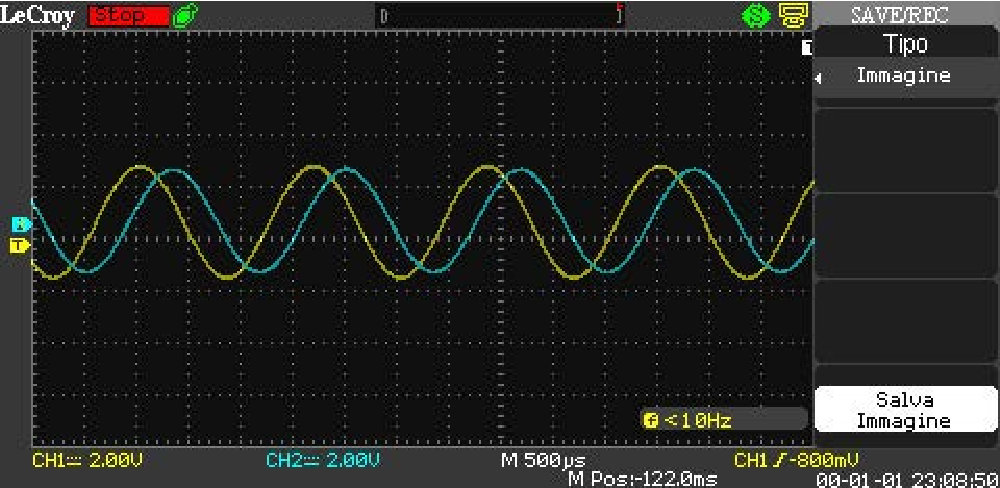
\includegraphics[width=0.7\linewidth]{imag/WA000018}
	\caption{Filtro passa-alto, valutazione sperimentale del guadagno}
	\label{fig:wa000018}
\end{figure}

Dall'oscilloscopio si legge che 
\[V_i = \SI{4}{\volt} \qquad V_{out} = \SI{4.4}{\volt}\]
Per cui 
\[G^{Re} = \dfrac{\SI{4.4}{\volt}}{\SI{4}{\volt}} = 1.1\]

\newpage

\begin{figure}[H]
	\centering
	\begin{subfigure}{.7\textwidth}
		\centering
		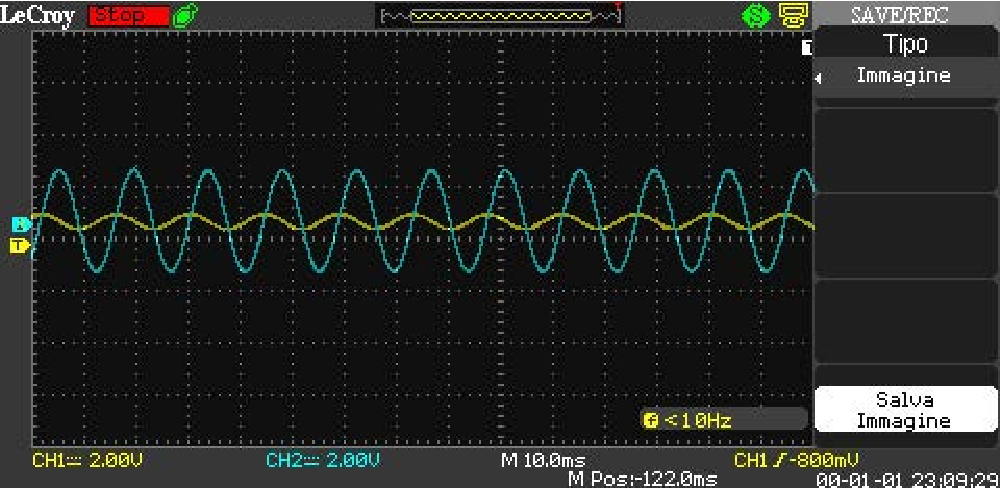
\includegraphics[width=.7\linewidth]{imag/WA000019}
		\caption{}
		\label{fig:wa000019}
	\end{subfigure}
	\hfill
	\begin{subfigure}{.7\textwidth}
		\centering
		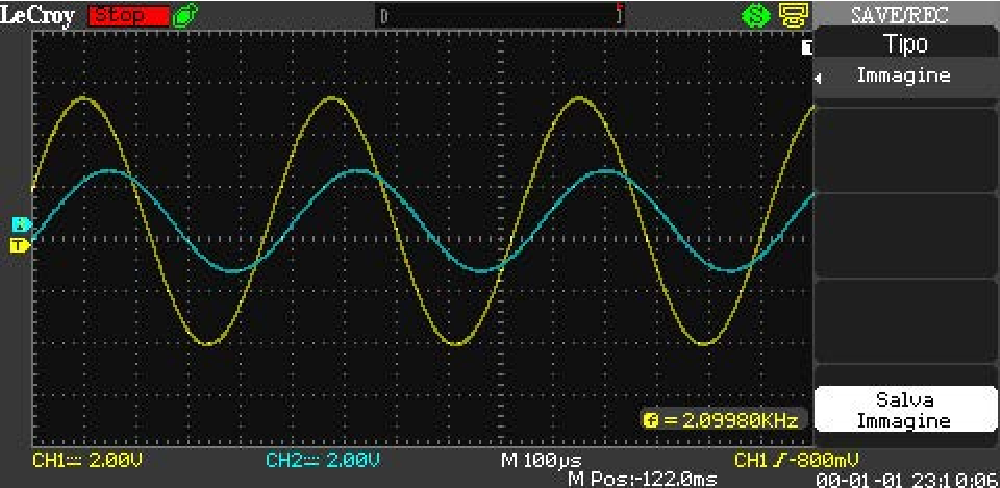
\includegraphics[width=.7\linewidth]{imag/WA000020}
		\caption{}
		\label{fig:wa000020}
	\end{subfigure}
	\hfill
	\begin{subfigure}{.7\textwidth}
		\centering
		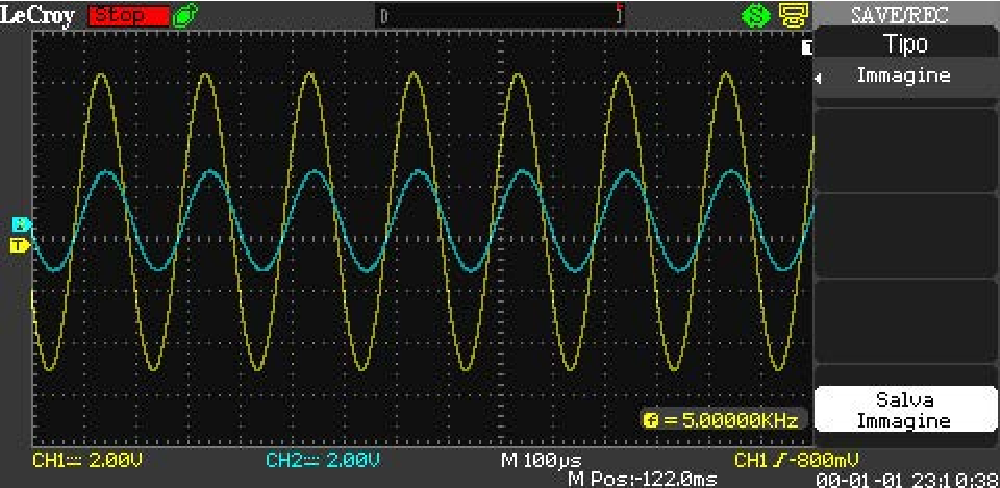
\includegraphics[width=.7\linewidth]{imag/WA000021}
		\caption{}
		\label{fig:wa000021}
	\end{subfigure}
	\hfill
	\begin{subfigure}{.7\textwidth}
		\centering
		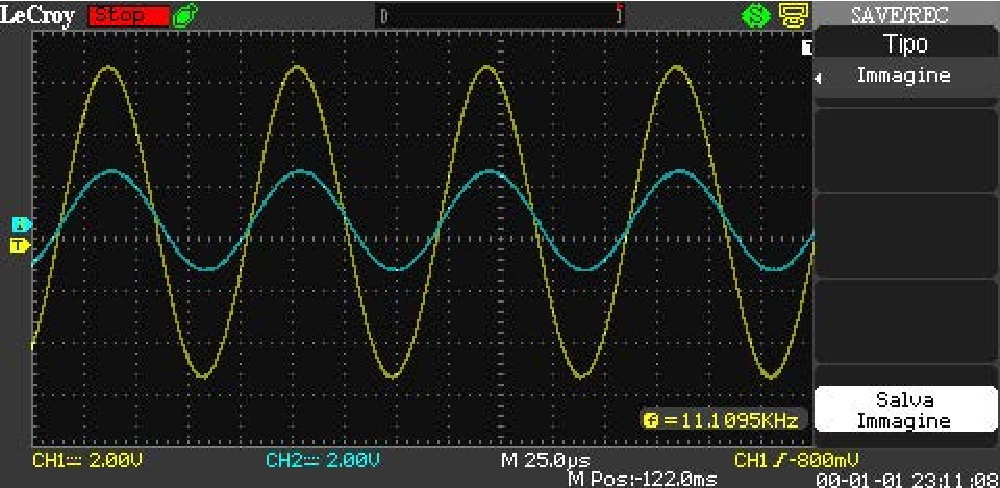
\includegraphics[width=.7\linewidth]{imag/WA000022}
		\caption{}
		\label{fig:wa000022}
	\end{subfigure}
	\caption{Grafici di cui calcolare la frequenza del segnale in ingresso ed il guadagno sperimentale}
\end{figure}
\newpage
\subsection{Quesito 3: calcolare la frequenza del segnale in ingresso}

\[f = \dfrac{1}{T}\]

La frequenza del segnale in \textcolor{cyan}{ingresso} è calcolabile dall'oscilloscopio. 

Si divide la base dei tempi per il numero di divisioni della singola unità, dopodiché si moltiplica questo valore per il numero di divisioni individuate all'interno dei due massimi o due minimi successivi e si ottiene il periodo.

\begin{itemize}
	\item \ref{fig:wa000019}
	\[\text{Base Tempi} = 2\dfrac{\SI{}{\milli\second}}{\text{div}}\]
	\[T = 7~\text{div}\cdot2\dfrac{\SI{}{\milli\second}}{\text{div}} = \SI{14}{\milli\second}\]
	\[f = \dfrac{1}{T} = \SI{0.071}{\kilo\hertz}\]
	
	\item \ref{fig:wa000020}
	\[\text{Base Tempi} = 20\dfrac{\SI{}{\micro\second}}{\text{div}}\]
	\[T = 24~\text{div}\cdot520\dfrac{\SI{}{\micro\second}}{\text{div}} = \SI{480}{\micro\second}\]
	\[f = \dfrac{1000}{T} = \SI{2.08}{\kilo\hertz}\]
	
	\item \ref{fig:wa000021}
	\[\text{Base Tempi} = 20\dfrac{\SI{}{\micro\second}}{\text{div}}\]
	\[T = 10~\text{div}\cdot520\dfrac{\SI{}{\micro\second}}{\text{div}} = \SI{200}{\micro\second}\]
	\[f = \dfrac{1000}{T} = \SI{5}{\kilo\hertz}\]
	
	\item \ref{fig:wa000022}
	\[\text{Base Tempi} = 5\dfrac{\SI{}{\micro\second}}{\text{div}}\]
	\[T = 18~\text{div}\cdot5\dfrac{\SI{}{\micro\second}}{\text{div}} = \SI{90}{\micro\second}\]
	\[f = \dfrac{1000}{T} = \SI{11.11}{\kilo\hertz}\]
\end{itemize}

\newpage

\subsection{Quesito 4: Costruire il grafico guadagno frequenza e calcolare sperimentalmente la frequenza di taglio}

Il guadagno del segnale  in ingresso è calcolabile dalla relazione (\ref{eq:2})
\[G = \left(1+\dfrac{R_f}{R_i}\right)\dfrac{\omega RC}{\sqrt{1+(\omega RC)^2}}\]
Dove 
\[\omega = 2\pi f\]
Allora per ogni immagine si avrà

\begin{table}[H]
	\centering
	\ra{1.3}
	\captionof{table}{Quesito 4} \label{tab:q4}
	\begin{tabular}{ccc}
		\toprule
		 \textbf{Figura}   & $\omega~\si{[1\per\second]}$ &   $G$    \\ \midrule
		\ref{fig:wa000019} &        \num{0.0446e4}        & $0.0891$ \\
		\ref{fig:wa000020} &        \num{1.3069e4}        & $1.5884$ \\ 
		\ref{fig:wa000021} &        \num{3.1416e4}        & $1.9058$ \\ 
		\ref{fig:wa000021} &        \num{6.9806e4}        & $1.9798$ \\ \bottomrule
	\end{tabular}
\end{table}

In questo modo si trova che il guadagno massimo del segnale è pari a 
\[G_{\max} = 1.9798\]
La frequenza di taglio si individua per una deamplificazione del guadagno massimo di  $\SI{3}{\decibel}$ per cui
\[G_{f_t} = \dfrac{1.9798}{\sqrt{2}} = 1.3999 \simeq 1.4\]
Graficamente si ottiene una frequenza di taglio sperimentale pari a
\[f_t^{Re} \simeq \SI{1.9}{\kilo\hertz}\]
Attraverso un codice Matlab è possibile individuare l'intersezione tra $G_{f_t}$ e la curva del valori per individuare con precisione la frequenza di taglio
\[f_t^{Re} = \SI{1.8275}{\kilo\hertz}\]
\newpage
\subsection{Grafici}
	Si riportano infine i grafici guadagno/frequenza, anche in scala semilogaritmica.

\begin{figure}[H]
	\hspace{-3cm}
	\centering
	\begin{subfigure}{.5\textwidth}
	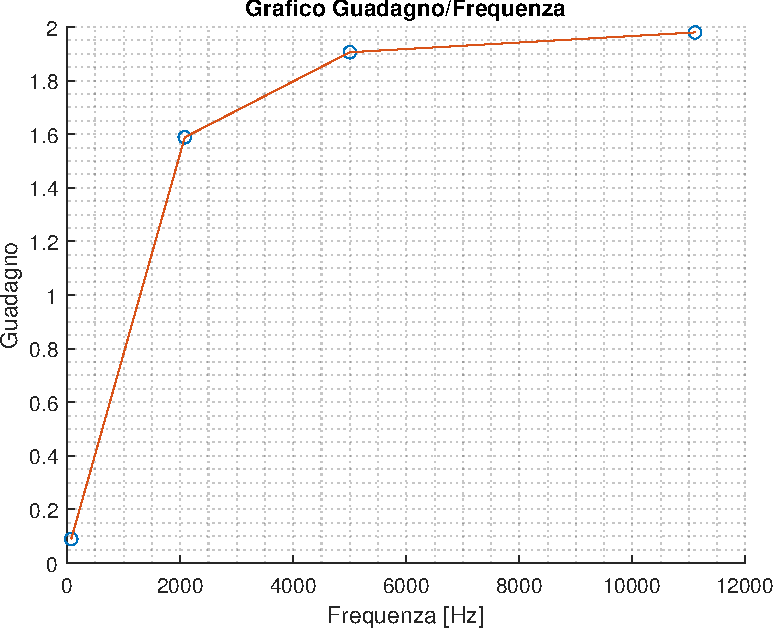
\includegraphics[width=\textwidth]{imag/Gf_nonlog}
	\caption{}
	\label{fig:gfnonlog}
	\end{subfigure}
	\hfill
	\begin{subfigure}{.5\textwidth}
	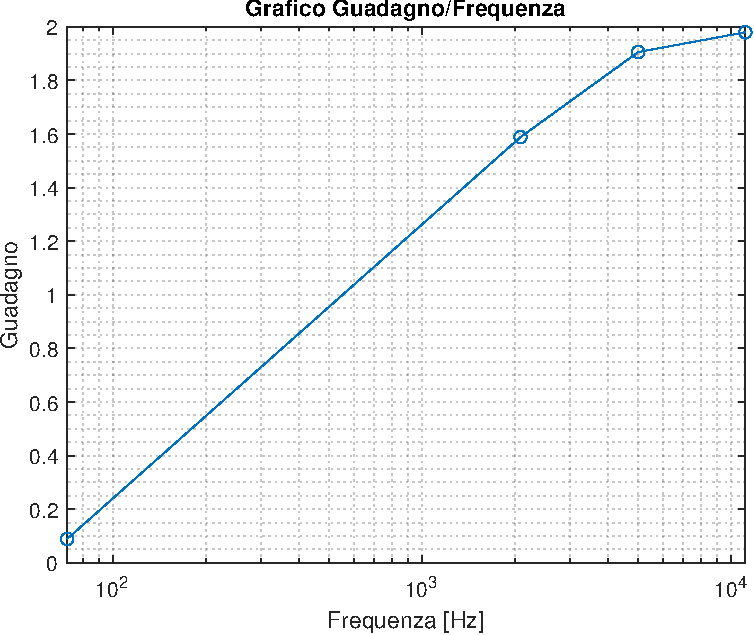
\includegraphics[width=\textwidth]{imag/Gf_semilog}
	\caption{}
	\label{fig:gflog}
	\end{subfigure}
\end{figure}
	\vspace{1.5cm}
	E i grafici che conducono all'individuazione della frequenza di taglio
	\begin{figure}[H]
		\hspace{-3cm}
		\centering
		\begin{subfigure}{.5\textwidth}
			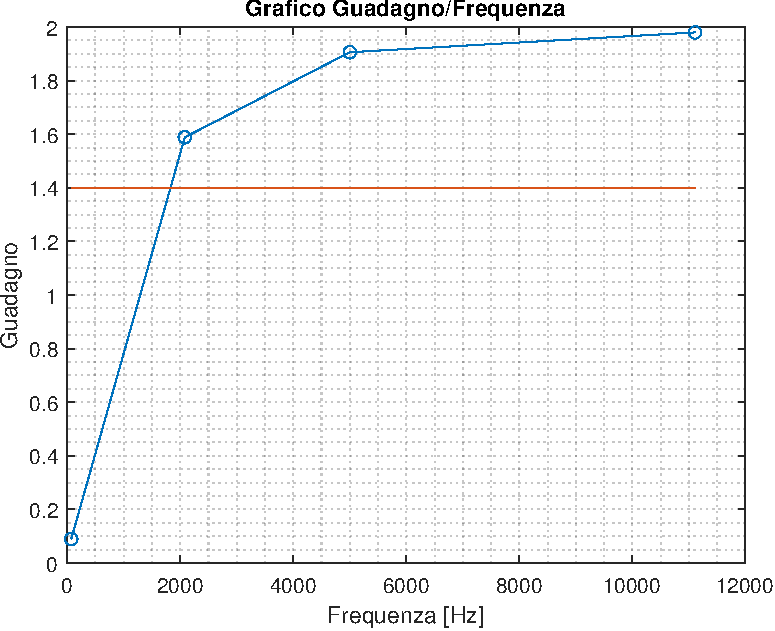
\includegraphics[width=\textwidth]{imag/Gf_deamp}
			\caption{}
			\label{fig:gfdeamp}
		\end{subfigure}
		\hfill
		\begin{subfigure}{.5\textwidth}
			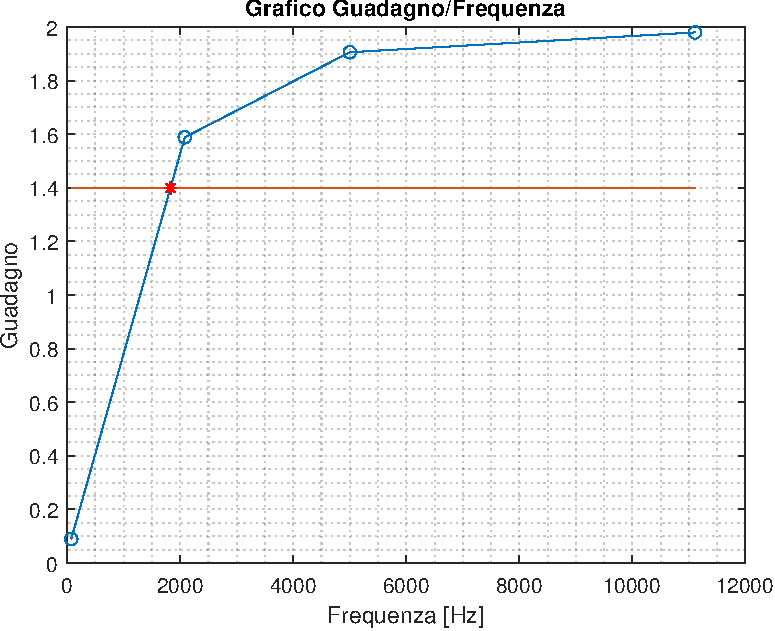
\includegraphics[width=\textwidth]{imag/Gf_ft}
			\caption{}
			\label{fig:gfft}
		\end{subfigure}
	\end{figure}
	
	\newpage
\newgeometry{top=0.5cm, bottom=0.5cm, left=0.5cm, right=0.5cm}		
	\section{Codice Matlab}
	\begin{verbatim}
		clear all
		close all
		clc
		format short
		
		tic
		%% Dati
		f = [71 2080 5000 11110]; % Hz Frequenza
		R = 1e3;
		C = 1e-7;
		
		% Calcolo del guadagno a partire dalla frequenza
		G0 = 2;
		omega = 2*pi.*f
		wRC = omega*R*C;
		den = sqrt(1+(wRC).^2);
		G = G0*(wRC./den)
		x = f; y = G;
		
		%% Grafico dati
		figure 
		plot(x,y, '-o')
		grid minor
		ylabel('Guadagno')
		xlabel('Frequenza [Hz]')
		title('Grafico Guadagno/Frequenza')  
		% Esportazione 
		ax = gca;
		% exportgraphics(ax,'Gf_nonlog.pdf','Resolution',300)
		
		%% Grafico semilogaritmico 
		figure 
		semilogx(x,y, '-o')
		grid minor
		ylabel('Guadagno')
		xlabel('Frequenza [Hz]')
		title('Grafico Guadagno/Frequenza semilogaritmico')  
		% Esportazione 
		ax = gca;
		% exportgraphics(ax,'Gf_semilog.pdf','Resolution',300)
		
		
		%% Individuazione della frequenza di taglio
		yft = G(4)/sqrt(2)
		xdb = [x(1) x(4)]; ydb = [yft yft];
		figure 
		plot(x,y, '-o')
		hold on
		plot(xdb,ydb)
		hold off 
		grid minor
		ylabel('Guadagno')
		xlabel('Frequenza [Hz]')
		title('Grafico Guadagno/Frequenza')  
		% Impostazione degli assi
		ax = gca;
		ax.XAxisLocation = 'origin';
		ax.YAxisLocation = 'origin';
		% Esportazione 
		% exportgraphics(ax,'Gf_deamp.pdf','Resolution',300)
		
		
		%% Intersezione 
		retta_db = polyfit(xdb, ydb,1);
		retta_necessaria = polyfit([x(1) x(2)], [y(1) y(2)], 1);
		
		x_intersect = fzero(@(x) polyval(retta_db-retta_necessaria,x),10e3);
		y_intersect = polyval(retta_db,x_intersect);
		
		figure 
		plot(x,y, '-o')
		hold on
		plot(xdb,ydb)
		plot(x_intersect,y_intersect,'r*')
		hold off 
		grid minor
		ylabel('Guadagno')
		xlabel('Frequenza [Hz]')
		title('Grafico Guadagno/Frequenza')  
		% Impostazione degli assi
		ax = gca;
		ax.XAxisLocation = 'origin';
		ax.YAxisLocation = 'origin';
		% Esportazione 
		% exportgraphics(ax,'Gf_ft.pdf','Resolution',300)
		
		disp(x_intersect)
		
		toc
	\end{verbatim}
	\restoregeometry
\end{document}

